\documentclass[smallextended,natbib]{svjour3}       % onecolumn (second format)
\usepackage{graphicx}
\usepackage[T1]{fontenc}
\usepackage{caption}
\usepackage{subcaption}
\usepackage{todonotes}
\usepackage{url}
\usepackage{lineno}
\linenumbers
\usepackage[hidelinks]{hyperref}
%\usepackage[showframe]{geometry}


\begin{document}
	
%opening
\title{Pikunda-Munda: Disappearance of Pottery Production in the Western Congo Basin at the End of the Early Iron Age}
%\titlerunning{Short form of title}        % if too long for running head

\author{Dirk Seidensticker}

\institute{Dirk Seidensticker \at
	Ghent University \\
	Department of Archaeology \\
	UFO, Sint-Pietersnieuwstraat 35 \\
	B-9000 Ghent \\
	\email{dirk.seidensticker@ugent.be}
}

\date{Received: date / Accepted: date}
% The correct dates will be entered by the editor

\maketitle

\begin{abstract}
The history of pottery-producing communities in Central Africa has long been seen as a study of its spread. While this process started about two-and-a-half millennia ago, it is often linked with the so-called 'Bantu Expansion'. Linguistic studies claimed substantial migratory events through the so-called 'Sangha River Interval', which mostly coincides with the Sangha river valley and the western part of the Congo Basin. This region is viewed as a 'gateway' communities followed to cross the equatorial rainforest during their spread south.

This paper presents novel data on the oldest widespread pottery from that region, the Pikunda-Munda style. Its emergence in the last century BCE is equally shrouded in secret as its disappearance in the fifth to sixth century CE. The latter coincides with a distinct period of low human activity (600--1000~CE) observed throughout Central Africa.

New research into the technological decisions or \textit{chaînes opératoires} of the potters' communities that produced Pikunda-Munda pottery revealed that they followed a distinct path, different from that in adjacent regions such as the Inner Congo Basin. Only regarding clay procurement and processing similar preferences for fluvial clay sources rich in sponge spicules can be seen. Drawing of a ring is the primary shaping or roughing-out technique and differences in how the bottoms were attached or closed indicate differences in trans-generational training networks among potters' communities of practice.

The disappearances of the Pikunda-Munda pottery mark an apparent abandonment of pottery production along the middle and lower Sangha river, with knowledge networks established earlier falling apart. There is little evidence for the persistence of the specific knowledge of Pikunda-Munda potters' communities. All groups encountered after the setback show evidence of them originating from groups found in the Inner Congo Basin. Potters' communities responsible for the Pikunda-Munda pottery were among those whose knowledge transfer was interrupted by the widespread setback in human activity observed throughout the wider region.

\noindent\textbf{Résumé} L'histoire des communautés productrices de poterie en Afrique centrale a longtemps été considérée comme une étude de sa propagation. Bien que ce processus ait commencé il y a environ deux millénaires et demi, il est souvent lié à la soi-disant \guillemotleft expansion bantoue\guillemotright. Des études linguistiques ont revendiqué des événements migratoires substantiels à travers le soi-disant \guillemotleft intervalle de la rivière Sangha\guillemotright, qui coïncide principalement avec la vallée de la rivière Sangha et la partie ouest du bassin du Congo. Cette région est considérée comme une «passerelle» des communautés suivies pour traverser la forêt tropicale équatoriale pendant leur propagation vers le sud.

Cet article présente de nouvelles données sur la plus ancienne poterie répandue de cette région, le style Pikunda-Munda. Son émergence au cours du siècle dernier BCE est également enveloppée de secret que sa disparition du 5e au 6ème siècle. Ce dernier coïncide avec une période distincte de faible activité humaine (600-1000 CE) observée dans toute l'Afrique centrale.

De nouvelles recherches sur les décisions technologiques ou l'opératoire de \textit{chaînes opératoires} des communautés des potiers qui produisaient la poterie Pikunda-Munda ont révélé qu'ils suivaient un chemin distinct, différent de celui des régions adjacentes telles que le bassin intérieur du Congo. Ce n'est qu'en ce qui concerne l'approvisionnement en argile et le traitement des préférences similaires pour les sources d'argile fluviale riches en épicules éponges. Le dessin d'un anneau est la principale technique de mise en forme ou de brouillage et les différences dans la façon dont les fonds ont été attachés ou fermés indiquent des différences dans les réseaux d'entraînement transgénérationnels parmi les communautés de pratique des potiers.

Les disparitions de la poterie Pikunda-Munda marquent un abandon apparent de la production de poterie le long de la rivière du milieu et du bas de Sangha, avec des réseaux de connaissances établis plus tôt en train de s'effondrer. Il existe peu de preuves de la persistance de la connaissance spécifique des communautés des potiers de Pikunda-Munda. Tous les groupes rencontrés après le revers montrent des preuves d'eux provenant de groupes trouvés dans le bassin intérieur du Congo. Les communautés des potiers responsables de la poterie Pikunda-Munda faisaient partie de celles dont le transfert de connaissances a été interrompu par le revers généralisé dans l'activité humaine observée dans toute la région plus large.

\keywords{Congo Basin \and Ceramics \and Knowledge transfer \and \textit{Chaîne opératoire} \and Middle Iron Age Hiatus}
\end{abstract}

\section{Introduction}\label{intro}

The spread of pottery-producing communities throughout Central Africa is regularly linked with the so-called 'Bantu Expansion' \citep{Bostoen.2018,Bostoen.2020}. The diversity of Bantu-languages spoken today is attributed to demic diffusion \citep{Pakendorf.2011,Bostoen.2022} and linguistic reconstructions of putative pathways favor rapid migrations through the equatorial rainforests of Central Africa \citep{Bostoen.2015,Grollemund.2015,Grollemund.2023,Koile.2022} (Fig.~\ref{fig:map}). To cope with the lack of historicity in modern language data, archaeological results are used to temporally 'calibrate' these migratory events. The resulting synopses are based on 'circular reasoning' \citep{Eggert.2016a}, usually involving the premise that the emergence of pottery in a given region equates with the arrival of Bantu-speakers \citep[355, 362, 364]{Bostoen.2015}.

These overreaching linguistic models still influence archaeological research \citep{Eggert.2005,Eggert.2012,Eggert.2016a} and force a stringent examination of (dis)-continuities within the archaeological record. The primary source of information on the material culture of communities living in Central Africa for the past 2.500 years are ceramic finds \citep{Eggert.2014}. Comprehensive sequences of pottery production are mainly known from the Congo Basin \citep{Wotzka.1995,Seidensticker.2021e} and Gabon \citep{Clist.20042005}. Research in other regions, such as Cameroon \citep{GouemGouem.20102011,NlendNlend.20132014}, yielded partial and regional sequences, often with missing details on the younger parts of the sequence. Despite disparate research focuses and lack of data, as vast regions have not been studied at all, a general trend with consecutive 'boom-and-bust' phases within the record of human activity in Central Africa can be reconstructed \citep{Oslisly.1998,Oslisly.2013,Oslisly.2013b,Saulieu.2017,deSaulieu.2021a,Seidensticker.2021}. A profound setback in human activity dates between the seventh to tenth century CE and divides the Early and Late Iron Ages. This widespread phase of 'low activity' \citep[Fig.~2]{Seidensticker.2021} questions the underlying assumption of historical linguists concerning a direct connection between early ceramic finds in a given region and modern Bantu-speech communities \citep{Grollemund.2015,Bostoen.2015} and, with it, the proposed reconstruction of the 'Bantu-Expansion' as a single migratory event \citep{Currie.2013,Koile.2022,Grollemund.2023}.

\begin{figure*}[!tb]
	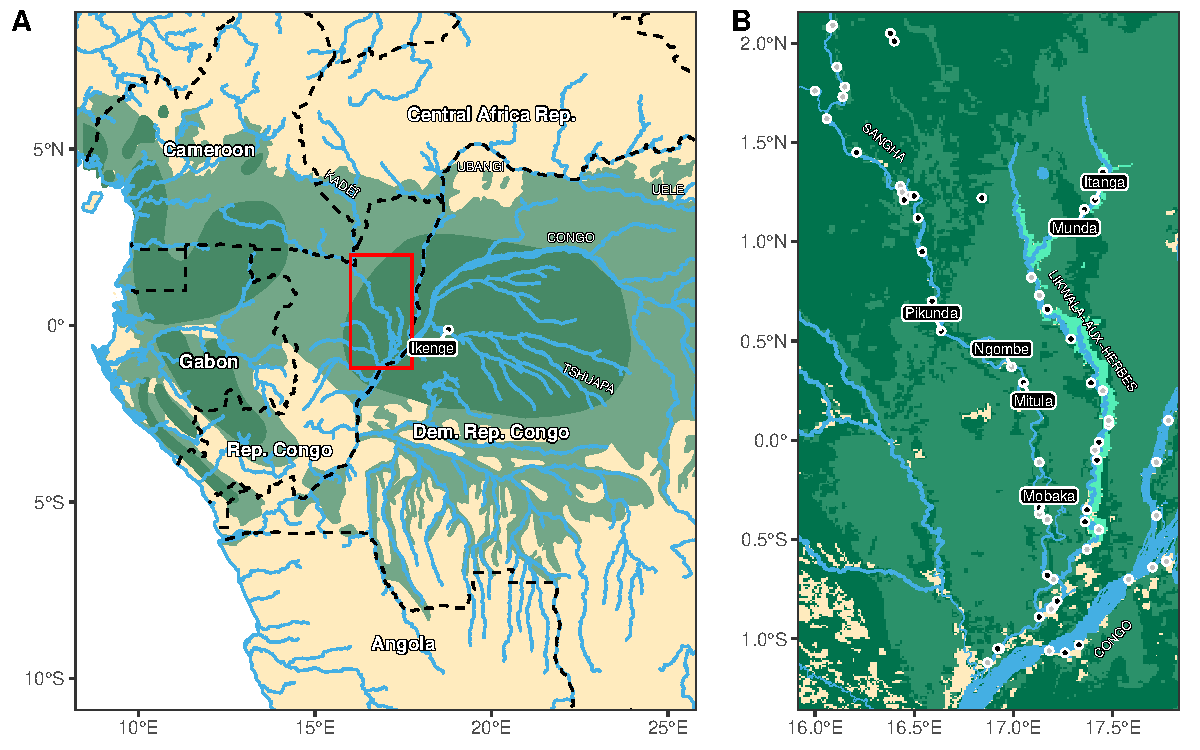
\includegraphics[width=\textwidth]{Fig_Map.pdf}
	\caption{Map of Central Africa (A) with the distribution of equatorial rainforest \citep{White.1983} (light green) and its putative distribution during the 1st millennium BCE \citep{Bremond.2017,Maley.2017} (dark green). The map of the study area along the rivers Sangha and Likwala-aux-Herbes (B) shows the distribution of landcover types based on satellite data \citep{Mayaux.2003}: closed evergreen rainforest vegetation (dark green), swamp forest (medium green), and swamp bush- and grassland (light green). Black dots show sites with Pikunda-Munda style pottery, while grey dots represent sites with other pottery finds \citep[11 Fig.~1, 119 Fig.~49]{Seidensticker.2021e}.}
	\label{fig:map}
\end{figure*}

\begin{figure*}[p]
	\centering 
	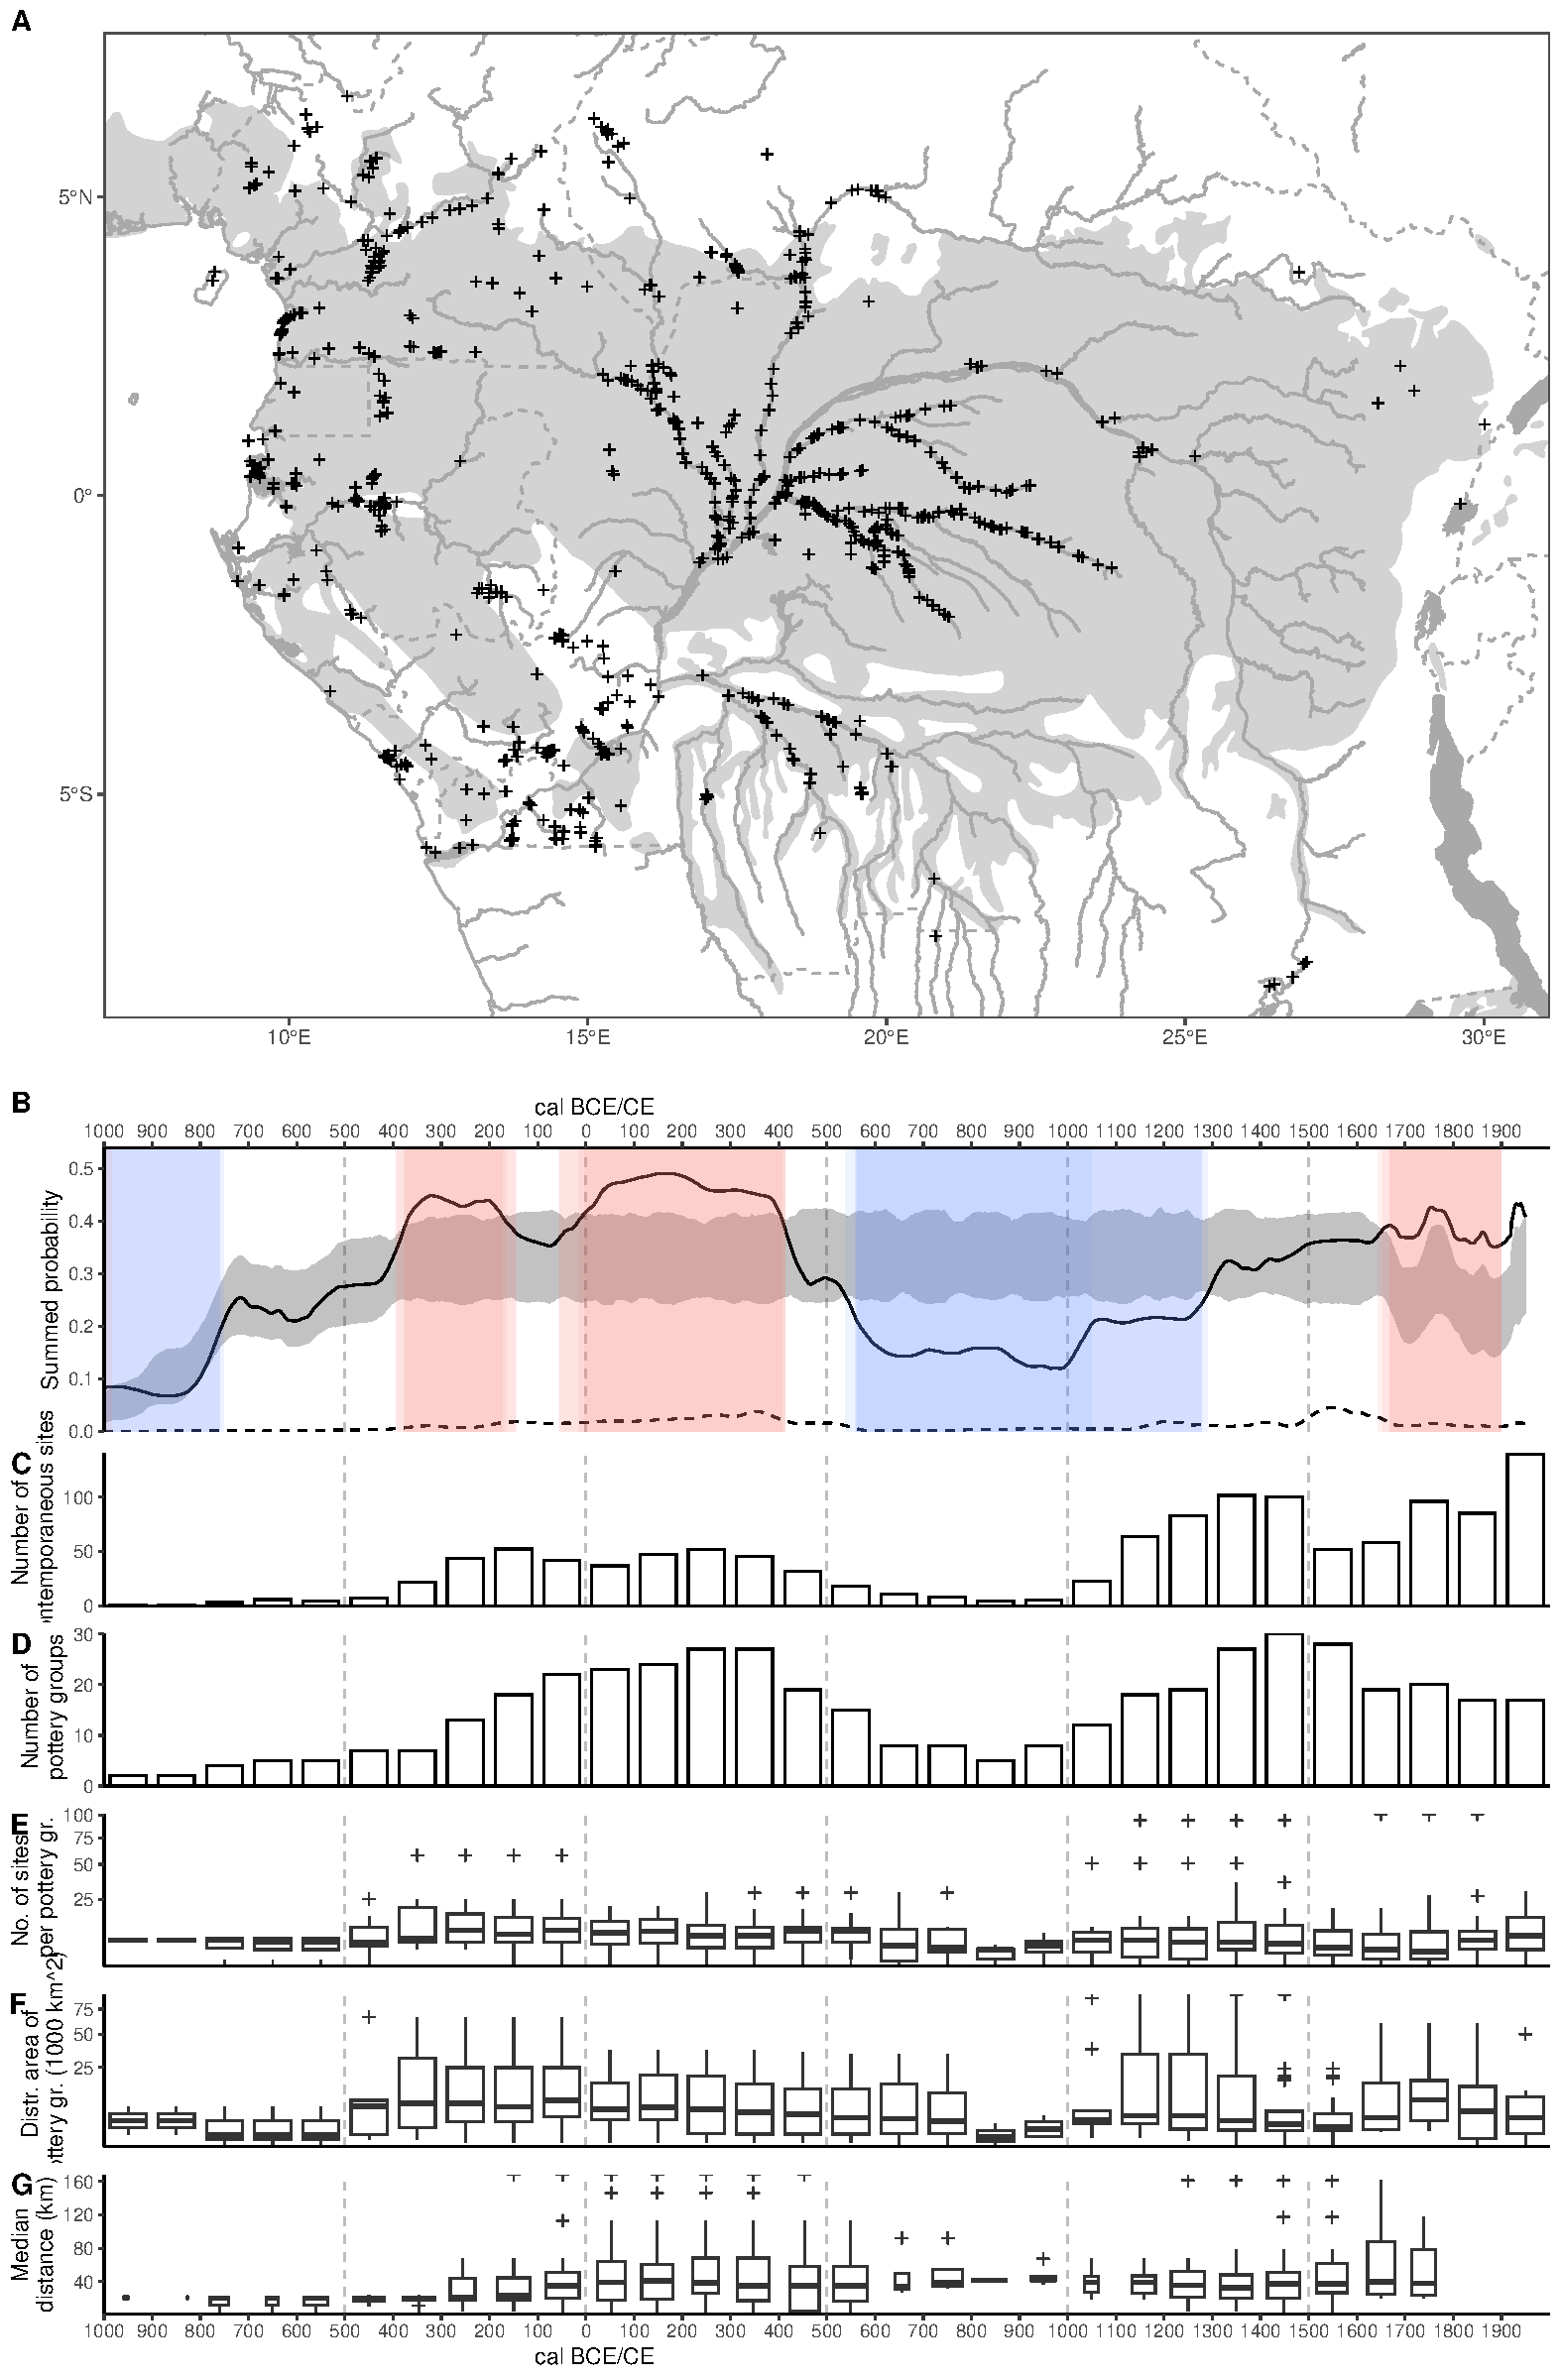
\includegraphics[width=\textwidth]{Fig_SPD.pdf}
	\caption{(Caption next page.)}
	\label{fig:spd}
\end{figure*}
\addtocounter{figure}{-1}
\begin{figure*}[t!]
	\caption{\textbf{A} Map of sites with radiocarbon dates or dated pottery finds. Light grey shading shows distribution of equatorial rainforest today \citep{White.1983}. \textbf{B} Temporal variation in the activity of ancient pottery-producing communities in the Congo rainforest over the past 3000 years \citep[regions A--H in][Fig.~2]{Seidensticker.2021}. Activity is discussed based on the SPD (full black lines) of all class Ia--c and IIa archaeological 14C dates (n = 1042) \citep{Seidensticker.2021f}, smoothed using a 60-year moving average. The dashed line represents the SPD for sites in the Sangha/Likwala-aux-Herbes region. Grey background shading represents the 95~\% uncertainty envelope of summed probability in a logistic model of hypothetical population growth drawn from the same 14C datasets \citep{Bevan.2022}. Color shading demarcates periods of more or less intense human activity, defined as time windows during which the observed SPD surpasses (red; 'heating up') or falls below (red, 'cooling down') one (light shading) or multiple (dark shading) growth models (based on 1000 MC runs). Note that the color scheme has been inverted compared to \citep[Fig.~2]{Seidensticker.2021} to correspond to other studies using the same methodology \citep{Crema.2016,Bevan.2017,Riris.2018,Riris.2019a,Brown.2019,Arroyo-Kalin.2021,deSouza.2021}. \textbf{C} Summed frequency of contemporaneous sites. The number of known sites for each pottery style was allocated for each century bin using a hypothesized function, in this case, Gaussian normal distribution, representing changes in saturation during the lifespan of a particular style \citep{Roberts.2012}. \textbf{D--G} Evolution of the numerical abundance and geographical distribution of pottery styles in the Congo rainforest \citep[Fig.~3]{Seidensticker.2021}. Abundance \textbf{(D)} is quantified as the number of pottery groups recorded within each century bin; spatial distribution is quantified as the number of sites where each pottery group is found \textbf{(E)} and by its total area of distribution \textbf{(F)}. \textbf{G} The median distances of sites pertaining to the same pottery group per century bin. Distances were calculated by constructing a network for each pottery group with more than five sites. For each group, sites were connected with their four nearest neighbors \citep{bivand2011spdep}.}
\end{figure*}

\begin{figure*}[p]
	\centering
	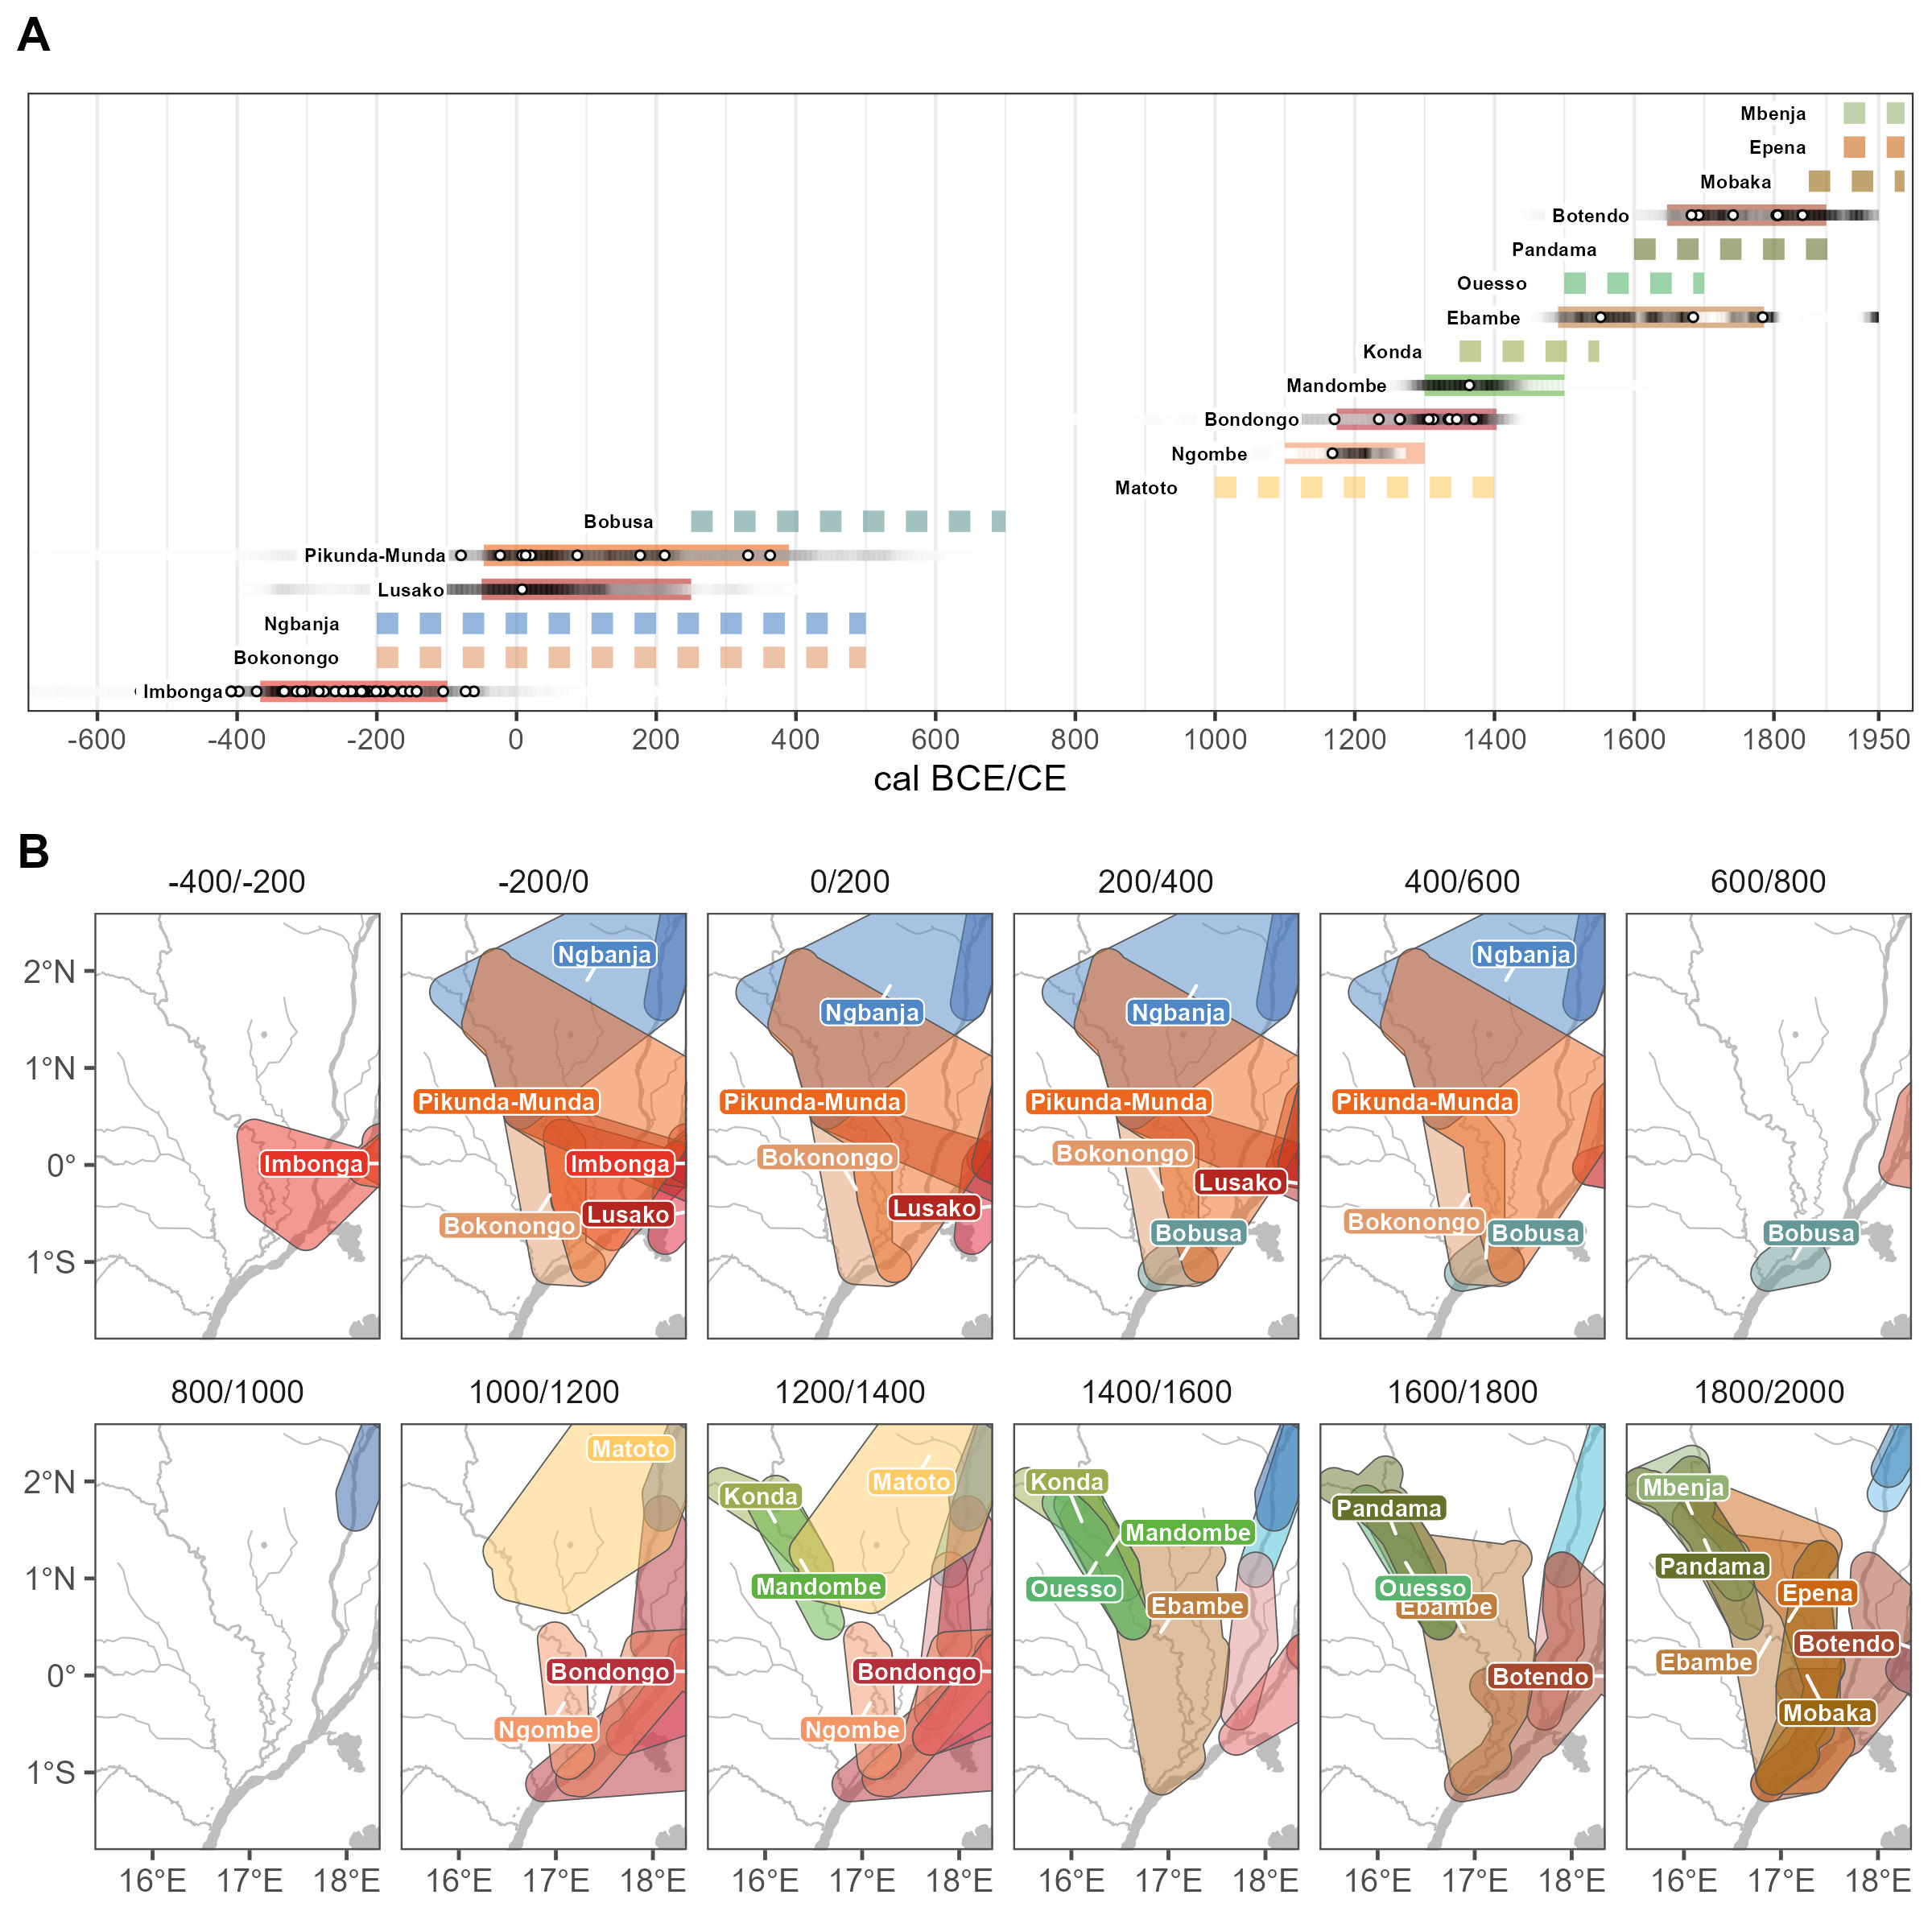
\includegraphics[width=\textwidth]{Fig_SanghaLikwala_Pottery_TimeSlices.pdf}
	\caption{Spatio-temporal distribution of known pottery styles in the Western Congo Basin (Fig.\ref{fig:sangahtypes}) over the past 2600 years. \textbf{A} Circles represent the highest probability of calibrated calendar age of each pottery-linked 14C date. The intensity of grey-shading is proportional to the summed probability of the calendar-age windows of all pottery occurrences by type. Colored bars represent the phase duration of radiocarbon dates pottery styles. For groups with more than two associated radiocarbon dates, the phases' median start and end dates were calculated using a Bayesian model \citep[Fig.~S1,Tab.~S1]{Crema.2021a,Crema.2021b,Seidensticker.2024}. Dashed colored bars indicate estimated bins derived from stylistic resemblance \citep[Data S2]{Seidensticker.2021}. \textbf{B} Time-sliced maps of occurrences of pottery styles in the Western Congo Basin. Negative numbers indicate calibrated ages BCE, while positive numbers represent calibrated ages CE. Extend per type was calculated as concave hull \citep{Gombin.2017} with a added buffer of 20~km. Colors correspond to \textbf{(A)}.}
	\label{fig:timeslicemaps}
\end{figure*}

The temporal variability in the activity of ancient pottery-producing communities over the past 3.000 years can best be derived from the available record of radiocarbon dates associated with properly described pottery finds \citep{Seidensticker.2021f}. An empirical summed probability distribution (SPD) computed from these dates, following a rigorous assessment of their 'chronometric hygiene' \citep{Napolitano.2019}, already shows a distinct bimodal pattern (Fig.~\ref{fig:spd}B: black line). To constrain the timing of distinct periods of over- or under-representation, the observed SPD can be compared with different models of hypothetical population growth using the rcarbon software \citep{Bevan.2022}. This analysis resulted in four successive periods during which the observed SPD either exceeds or falls short of the population growth trends predicted by four distinct models (Fig.~\ref{fig:spd}B: blue and red shading, respectively). A logistic growth model (Fig.~\ref{fig:spd}B: grey envelope) is probably most pertinent in the context of the 'Bantu-Expansion', which is often presented as a large-scale and exceptionally rapid process followed by a continuous presence of Bantu-speaking people after the initial expansion \citep{Pakendorf.2011,Grollemund.2015,Bostoen.2015,Bostoen.2022,Koile.2022}. Additionally, the empirical SPD was also tested against a 'uniform' model, representing a stable system, and two growth models; one representing 'linear' growth, while the second represents a scenario with 'exponential' growth. While \citet{Clist.2023a} deem various research biases impeding robust modeling, the combination of all four models provides a clear signal for a distinct setback in human activity throughout the Central African equatorial rainforest, but not complete abandonment, between the seventh and tenth century CE \citep{Seidensticker.2021f}, challenging assumptions of direct continuity between early and modern potters' communities. 

Additional corroboration of these findings come from the meta-data of known pottery groups in Central Africa. The summed frequency of contemporaneous sites modeled for each known pottery style using a Gaussian normal distribution \citet{Roberts.2012} shows a distinct, bimodal trend as well (Fig.~\ref{fig:spd}C): a surge in the number of sites in the second half of the 1st millennium BCE, that led into a stagnation phase, which is followed by a decline. The number of sites only increases after 1.000 CE again. The same pattern can be observed when viewing the number of pottery styles through time (Fig.~\ref{fig:spd}D). The 'evolution' of pottery producing communities in Central Africa confirms the temporal fluctuations reflected in the supra-regional SPD of archaeological radiocarbon dates (Fig.~\ref{fig:spd}B) and unveils a two-phase pattern during both the Early and Late Iron Age periods. Each starts with a phase of expansion during which stylistically homogeneous pottery groups became widely distributed and ends with a phase of high activity characterized by increasing abundance of local pottery styles reflecting a process of regionalization \citep{Seidensticker.2021}. 

\begin{figure*}[!tb]
	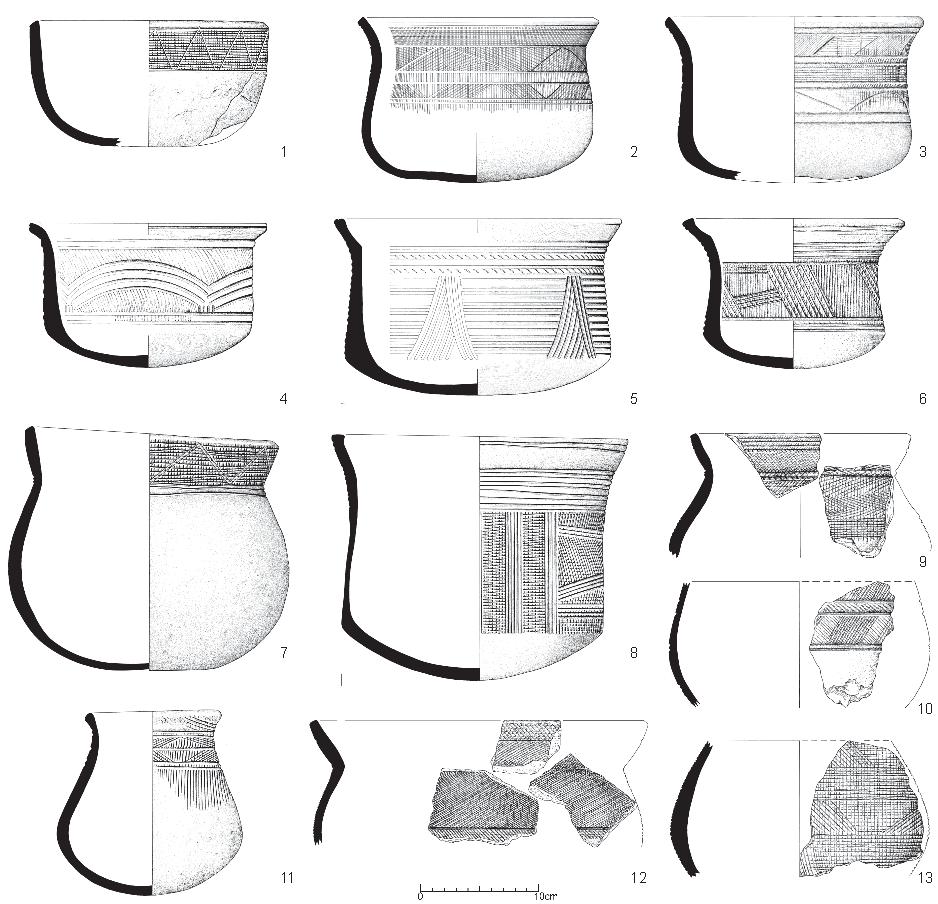
\includegraphics[width=\textwidth]{Fig_PKMvessels.pdf}
	\caption{Characteristic spectra of vessels associated with the Pikunda-Munda style group. (Drawings: Rita Vollbracht)}
	\label{fig:pkmtypes}
\end{figure*}

The history of localized discontinuities among potters' communities can be described best in the western Congo Basin. The Pikunda-Munda style \cite[114--120]{Seidensticker.2021e}, first described by Manfred \citet{Eggert.1992,Eggert.1993} following fieldwork of the \textit{River Reconnaissance Project} in 1987, is the oldest widespread pottery found throughout the western Congo Basin (Fig.~\ref{fig:map}B; \ref{fig:timeslicemaps}). Only isolated finds of vessel parts associated with the Imbonga style from Mobaka and Mitula are older \cite[Fig.~\ref{fig:map}B;][169--172]{Seidensticker.2021e}. The distribution area of the Pikunda-Munda style is about 300 to 150~km large (black dots in Fig.~\ref{fig:map}B). Its main characteristics, or type-species, are wide, open-mouthed bowls with approximately parallel or concave sides, flared rims, and rounded bases (Fig.~\ref{fig:pkmtypes}). The general ornament scheme is based on linear elements produced through incision and grooving. Rocker-stamp decoration is occasionally present. Stylistically, it shows some similarities to contemporaneous groups of the Inner Congo Basin, such as the styles Lokondola, Lusako, Lingonda, and Bokuma \citep[107]{Wotzka.1995}. The available data point towards an interpretation in which the Pikunda-Munda style is a rather distant sub-stream of the Equator-Co style tradition and no fully independent entity \citep[192]{Seidensticker.2021e}. Based on the current knowledge of the region's archaeology, the style has no known predecessor in the western Congo Basin. It is furthermore remarkable that its characteristics vanish from the region in the fifth to sixth century CE. All subsequent pottery styles found within the distribution area of the Pikunda-Munda style have their origin either in the Equator-Co style tradition of the Inner Congo Basin \citep[222--224 Fig.~4, 273]{Wotzka.1995} or the Ngoko style tradition originating in south-east Cameroon \citep[Fig.~\ref{fig:timeslicemaps};][189--192]{Seidensticker.2021e}.

Thus, the settlement history of the western Congo Basin follows the general bimodal picture \citep{Seidensticker.2016b,Seidensticker.2021e,Seidensticker.2024} and the disappearance of pottery in the region after the fifth to sixth century CE underlines the inaccuracies actuated by simple historical projections of modern language data \citep{Grollemund.2015,Bostoen.2015,Koile.2022}. It further raises the question of what happened to communities living in the western Congo Basin at the end of the Early Iron Age.

\section{Materials and Methods}\label{materials}

\subsection{Pikunda-Munda Style Pottery}

The Pikunda-Munda pottery style, among the oldest along the rivers Sangha and Likwala-aux-Herbes, was first described by \citet{Eggert.1992}. Pottery of this style has been excavated at the two eponymous sites: Pikunda along the middle Sangha river and Munda on the upper Likwala-aux-Herbes river (Fig.~\ref{fig:map}B). In total, 37 complete vessels, or sufficiently preserved pieces allowing reconstruction of the entire profile, belonging to the Pikunda-Munda style have been uncovered \citep[114--115]{Seidensticker.2021e}. The pottery is known from seven sites in the western Congo Basin \citep[119--120 Fig.~49]{Seidensticker.2021e}. With some reservations, sherds from another 24 sites, including one in the Inner Congo basin, can be assigned to the Pikunda-Munda style (Fig.~\ref{fig:map}B; \ref{fig:timeslicemaps}). The defining inventories are three pits excavated in 1987: pit B in trench PIK~87/1 at Pikunda \citep[288--300]{Seidensticker.2021e} and two ceramic depositions in pits from Munda labeled MUN~87/2-1-1 and MUN~87/2-1-3 \citep[321--335]{Seidensticker.2021e}. The characteristic open-mouthed bowls with flared rimes, cylindrical or concave upper parts and rounded bases \citep[311-314]{Eggert.1993} can be further divided into two sub-groups: one is characterized by a rounded transition from the wall to the base (Fig.~\ref{fig:pkmtypes}.2--3), while the second group shows a distinct carination in the profile (Fig.~\ref{fig:pkmtypes}.4--6,8). Bowls of the former type were exclusively found within the older infill of feature MUN~87/2-1-1 as well as the inventory from the neighboring pit MUN~87/2-1-3. Bowls with the characteristic carination were found in the upper infill of MUN~87/2-1-1 and in pit B of trench PIK~87/1 at Pikunda \citep[115--117]{Seidensticker.2021e}. Lesser represented among the complete vessels, but present in equal numbers in the overall inventory, are slightly globular vessels with everted rims (Fig.~\ref{fig:pkmtypes}.7,9--13). Decorations consist of linear elements produced utilizing incision or grooving and rocker-stamping with a comb \citep[362 App.~4.12]{Seidensticker.2021e}. Nine conventional radiocarbon dates \citep[117 Fig.~48, 355--356 App.~2]{Seidensticker.2021e} and one newer AMS date \citep[Tab.~2: RICH-30864]{Seidensticker.2024} date the Pikunda-Munda style between the second and first century BCE to fifth century CE.

This study focused on 39 vessel units of the Pikunda-Munda style (Tab.~\ref{tab:samples}). Eight originate from the pit at Pikunda (B in PIK~87/1), while the inventories of the two pits at Munda are represented by 13 (MUN~87/2-1-1) and 17 (MUN~878/2-1-3) vessel units, respectively. A single Pikunda-Munda sherd found in secondary depositon in the modern pit PIK~87/2 at Pikunda was also included. The main goal of the re-examination was to ameliorate a preliminary study concerning the \textit{chaîne opératoire} of potters' communities, which only included six vessels of the Pikunda-Munda style \citep[45--73]{Seidensticker.2021e}.

\begin{table*}[p]
	\centering
	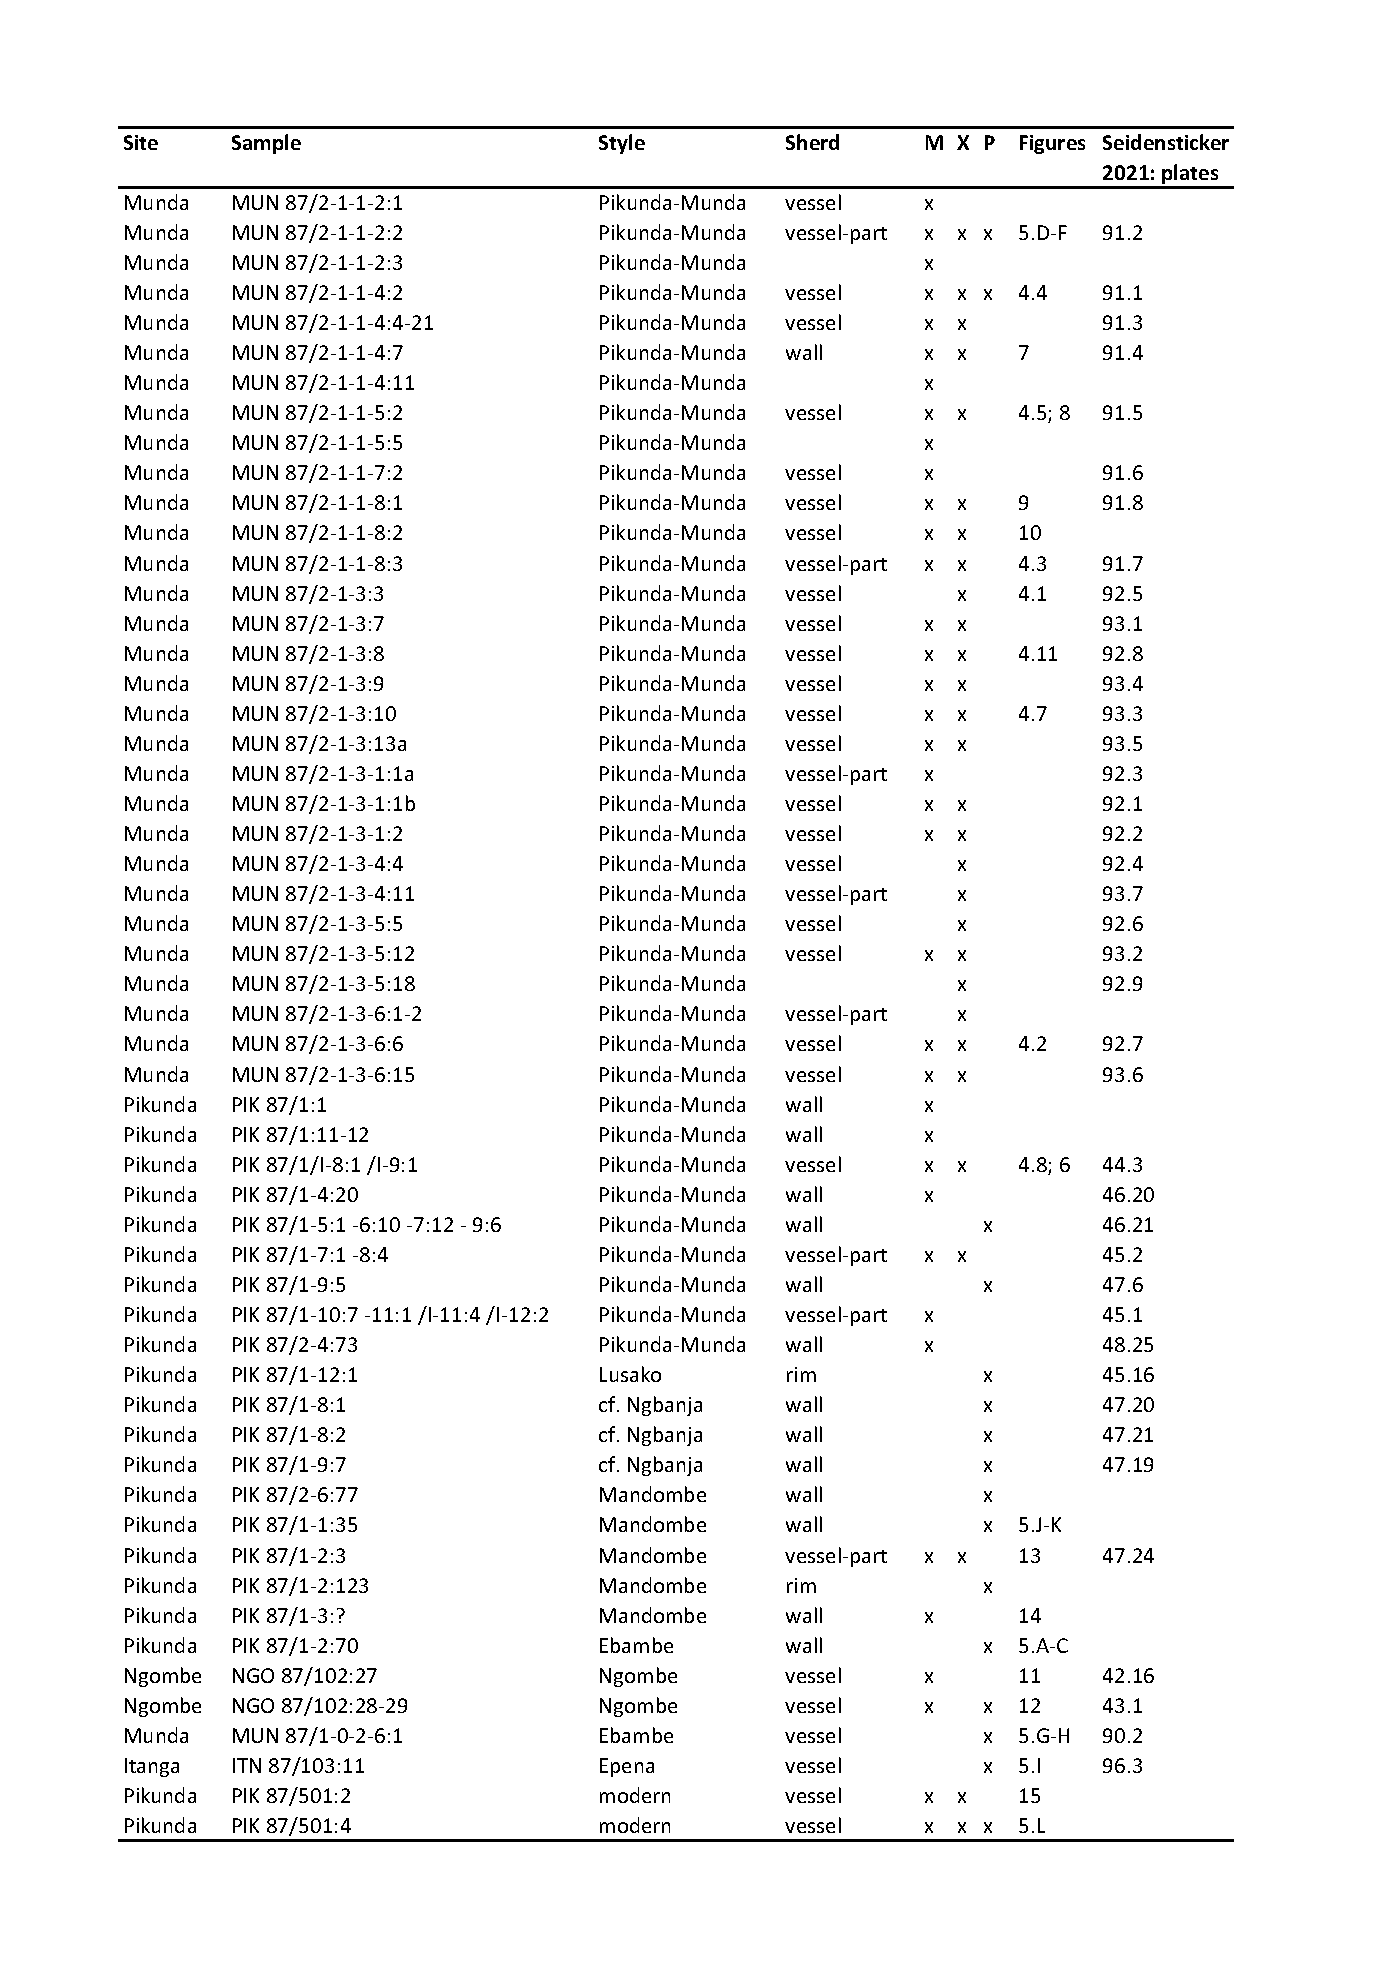
\includegraphics[height=.88\textheight]{Tab_Samples.pdf}
	\caption{List of samples included in this study and applied methods. Type of sherds are seperated for complete or nearly complete vessels, vessel parts of which considerable parts are missing, but the entire profile from the rim to the base can be reconstructed, and wall fragments with either the rim or base missing. The samples were subjected to macro-analysis of surface traces (M), X-raying (X), and petrographic analysis (P).}
	% vessel - nearly complete; vessel-part - profile from rim to base but bigger missing parts; wall - rim or base missing
	\label{tab:samples}	
\end{table*}

\subsection{Pottery Fabrics and Thin-Cection Petrography}

Previous research established a reference system with nine primary macroscopic ceramic fabrics \cite[60--69]{Seidensticker.2021e}. This system grouped sherds according to criteria observable without technical means other than a magnifier. Each major group was conceptualized as a putative 'recipe' prehistoric potters followed while sourcing and preparing used raw materials, most importantly clay and temper agents \citep[49]{Lange.2006}. The main characteristics to differentiate 'fabrics' \citep[cf.][38--51]{Riemer.2011} were the composition and texture of the clay matrix and non-plastic components as well as the firing color \citep[34]{Nordstrom.1972}. Differences within the nine main fabrics resulted in a general reference system of 27 macroscopic ceramic fabrics for the western and northern Congo Basin \citep[62--65 Tab.~11]{Seidensticker.2021e}. Some main macroscopic fabrics correlate with stylistic groups \cite[69 Tab.~12]{Seidensticker.2021e}. For example, all investigated sherds that are either part of the West tradition of the Equator-Co style tradition of the Inner Congo basin \citep[221--222 Fig.~4]{Wotzka.1995} or stylistically closely related to those are part of the same macroscopic fabric group, labeled 'fabric 1'. This fabric is characterized by whitish firing colors and almost no visible non-plastic particles. Pottery from sites along the Likwala-aux-Herbes and lower Sangha river are almost exclusively part of this fabric \cite[67 Fig.~21]{Seidensticker.2021e}. Thus, in this region, potters followed the same 'recipe' for sourcing and preparing clay since the onset of pottery production in that region in the last centuries BCE. The available qualitative descriptions of the technological aspects of the pottery styles in the Inner Congo Basin by \citet[59--210]{Wotzka.1995} indicate that nearly all styles in the western parts of this region would be assigned to the same fabric group 1 as they display comparable characteristics. Only styles that date after the fifteenth century CE and are part of the Tshuapa, Maringa, or northern style tradition in the eastern part of the Inner Congo Basin show higher concentrations of quartz inclusions and would thus be grouped in macroscopic fabric 4 \citep[62--65 Tab.~11]{Seidensticker.2021e}.

To further elaborate on this preliminary and superficial analysis, a comprehensive study of the mineralogical compositions of pottery sherds from the Congo Basin was started. For this paper, four thin-sections from ceramics of the Pikunda-Munda style (Fig.~\ref{fig:thinsections}A--F) as well as nine thin-sections from younger pottery from the two main sites Pikunda and Munda (Fig.~\ref{fig:thinsections}G--L) were studied (Tab.~\ref{tab:samples}). The petrographic analysis was conducted using an Olympus BX41 microscope, and the description and interpretation of observations were based on established reference works regarding ceramic petrography \citep{MacKenzie.2017,Quinn.2022}. 

\subsection{Macro-Traces and X-Radiographs}

The shaping technique is the second aspect of the \textit{chaîne opératoire} of Pikunda-Munda potters under investigation in this paper. The shaping process can be sub-divided into two phases: the forming or roughing-out phase, henceforth referred to as the 'primary shaping technique', and the subsequent 'secondary' shaping technique \citep{Shepard.1956,Rye.1981,LivingstoneSmith.2007a,LivingstoneSmith.2010c}. Distinct actions of the potter during the shaping process can be deduced through surface features such as fissures, cracks, or breaks and their pattern, defective joints, as well as variations in the texture of the surfaces. Systematically spatially co-occurring features, systematized as configurations following \citet{LivingstoneSmith.2007a} as well as \citet{LivingstoneSmith.2010c}, are physical remnants of technical behaviors. These are compared and interpreted in reference to available ethnographic descriptions of the potting practices in the immediate study area \citep{Eggert.1980c,Eggert.inVorb.}, as well as from the wider region \citep{Gosselain.1992,Gosselain.2002,Gosselain.1997,LivingstoneSmith.2007b,LivingstoneSmith.2010a,LivingstoneSmith.2016,LivingstoneSmith.2009,LivingstoneSmith.2010c} and other parts of Africa \citep{Gallay.1998,GasparDaSilva.2005,Gosselain.2005,Gosselain.2006,LivingstoneSmith.2007a,Mayor.2011a,Gosselain.2014}.

A preliminary study on 28 vessels from the western and northern Congo Basin, including six vessels of the Pikunda-Munda style, could identify three main groups of vessels sharing observed macro-traces and surface features \citep[45--60,69--73]{Seidensticker.2021e}. The present study included 39 vessel units of the Pikunda-Munda style alone (Tab.~\ref{tab:samples}).

The study of macro-traces was supplemented through x-radiographs that offered insight into the internal micro-structure of the vessels \citep{Stevenson.1953,Rye.1977,Vandiver.1987}. Radiographs of 26 vessels pertaining to the Pikunda-Munda group were produced at the Royal Museum for Central Africa (RMCA). The bulk of these vessels originated from the two neighboring pit features MUN~87/2-1-1 (n=8) and MUN~87/2-1-3 (n=16) at Munda on the Likwala-aux-Herbes river. Only two vessel units from the pit PIK~87/1 were sufficiently big enough to the radiographed.

\section{Results}

\subsection{Macroscopic and Petrographic Fabrics}

\begin{figure*}[!tb]
	\includegraphics[width=\textwidth]{Fig_Thinsections.pdf}
	% A-C: PIK 87/1-2:70 #55
	% D-F: MUN 87/2-1-1-2:2 #3
	% G-H: MUN 87/1-0-2-6:1 #17
	% I: ITN 87/103:11 #21
	% J-K: PIK 87/1-1:35 #11
	% L: PIK 87/501:4 #57
	\caption{Photomicrographs of ceramics from Pikunda (A--C, J--L), Munda (D--H) and Itanga (I) (\textit{cf}. Fig.~\ref{fig:map}B) dating into the Early (A--F) and Late Iron Age (G--L) illustrating the main petro-fabrics encountered (A--B,D--E,G--J in plain-polarized light [PPL]; C,F,K--L in cross-polarized light [XPL]). Pikunda-Munda pottery (A--F) is unanimously produced using fluvial clays rich in sponge spicules (A--H). Samples from Pikunda dating into the Late Iron Age were systemically produced using clays void of sponge spicules (J--L). Additional features include clay pellets (B--C) and clay mixing (I).}
	\label{fig:thinsections}
\end{figure*}

Previous studies \citep[60--69]{Seidensticker.2021e} established that Pikunda-Munda ceramics unanimously show the same macroscopic fabric: a fine clay paste usually dark or whitish in colour with no or very few macroscopic inclusions. The petrographic analysis corroborated this. Four sherds of vessels of the Pikunda-Munda style group showed strong similarities (Fig.~\ref{fig:thinsections}A--F). The petro-fabric is based on fine clays showing no or very little birefringence (Fig.~\ref{fig:thinsections}C,\ref{fig:thinsections}F). Its main feature is large quantities of sponge spicules. These appear as elongated isotropic rods in plane-polarized light (PPL; Fig.~\ref{fig:thinsections}A,E,H) and are the remains of the micro-sized, siliceous skeletons of freshwater sponges. Sponges, known as Cauixi in Amazonia, are known to have been added as temper agents to pre-Columbian pottery in the Amazon Basin \citep{Linne.1932,Linne.1957,Costa.2004,Rodrigues.2017,Villagran.2022}, as well as the Orinoco river valley \citep{LozadaMendieta.2019} and in the Paraná river valley \citep{Ottalagano.2016}. They are known to improve the mechanical properties of the vessels after firing by increasing mechanical rigidity \citep{Natalio.2015}. In Africa, as in other parts of the world \citep{Cordell.1993,Bloch.2019}, they indicate the use of lacustrine or fluvial clay sources. Sponge spicules rich pottery is rarely documented in pottery from sub-Saharan Africa though. Some examples are known from Mali \citep{Brissaud.1986,Mcintosh.1989,Nixon.2017}, Sudan \citep{Adamson.1987} and the great lakes region of East Africa \citep[185]{Ashley.2005}. Contrasting these few empirical evidence against the wide usage of fluvial clay's among modern potters communities in Africa \citep[19 Map~1]{Drost.1967} exemplifies the novelty of the observation of their wide presence in the Congo Basin. A lack of observed gemmules in the thin sections hampers species identification. A synthesis of spongillofauna in Africa by \citet{Manconi.2009} offers some potential candidates: \textit{Metania pottsi} is widely distributed in the region, but spicules often show conules on the surface, and the species is best identified based on their gemmuloscleres \citep[38--47]{Manconi.2009}, which are lacking in the archaeological samples. Other species with matching features are either not documented in the western Congo Basin, such as \textit{Eunapius nitens} \citep[149--151]{Manconi.2009}, which shows very similar spicules, or are poorly documented, such as \textit{Trochospongilla philottiana} \citep[198--199]{Manconi.2009}. 

The quartz fraction observed within this fabric consists of sub-angular mono-crystalline grains that are interpreted as natural components of the source clays (Fig.~\ref{fig:thinsections}C,F). Occasionally, clay pellets (Fig.~\ref{fig:thinsections}C) and evidence for clay mixing (Fig.~\ref{fig:thinsections}A,I) were observed. Clay mixing results in varying 'optical activity' under cross-polarized light (XPL) \citep{Whitbread.1986}. In general, only very limited or no birefringence was observed. One sherd from Munda on the upper Likwala-aux-Herbes river (Fig.~\ref{fig:thinsections}D) showed a zonation separating a clay matrix without birefringence from one with reddish interference colours and slight birefringence. The petro-fabric corresponds to the described fine macroscopic fabric 1 \citep[60--69]{Seidensticker.2021e}. 
 
While the selection of fluvial clays, rich in sponge spicules and an absence of any additional tempering, can be considered a distinct characteristic among Pikunda-Munda potters, substantial changes can be observed in later times among potters' communities along the middle to upper Sangha river versus those on the lower reaches of the Sangha and along the Likwala-aux-Herbes river. At Pikunda on the Sangha river, potters' approached distinctly different clay sources and tempered their clays \citep{Seidensticker.2016b,Seidensticker.2020}. There are no indications that fluvial clays rich in sponge spicules were used further. The late Iron Age sherds from Pikunda show distinct birefringence \citep[Fig.~\ref{fig:thinsections}K--L;][131--141]{Stoops.2021}. The mineral component is considerably different from that seen in the thin-section of the Pikunda-Munda sherds: quartz grains are bigger, more angular and occasionally, multi-crystalline rock fragments can be observed (Fig.~\ref{fig:thinsections}K). Runiquartz \citep[673 Fig.~6]{Marcelino.2018} is regularly present as well (Fig.~\ref{fig:thinsections}L). They indicate weathering of the quartz and, thus, a highly altered environment. The sherds also contain opaque components (Fig.~\ref{fig:thinsections}J--K), reminiscent of iron-rich minerals potentially related to lateritic soil formation processes \citep[351--352]{Scheffer.2010}. Occasionally, organic inclusions are visible. These observations indicate that potters of the late Iron Age potentially preferred clay sources that show some relation to soil formation processes and tempered those clays with mineral components and organics.

On the lower Sangha and the Likwala-aux-Herbes river, on the other hand, Late Iron Age potters still use similar or the same fluvial clay sources prevalent in the Early Iron Age pottery. The pottery of the younger styles Ngombe, Ebambe, Epena, and Mobaka (Fig.~\ref{fig:timeslicemaps}) all show the same macroscopic fabric 1 \citep[69 Tab.~12]{Seidensticker.2021e}, which corresponds with the petro-fabric rich in sponge spicules, indicating the use of fluvial clays. The concentric orientation of sponge spicules in a sherd from Munda (Fig.~\ref{fig:thinsections}G) indicates either clay mixing or shaping by coiling.

\subsection{Shaping techniques}

\begin{figure*}[!tb]
	\noindent\begin{minipage}{\textwidth}
		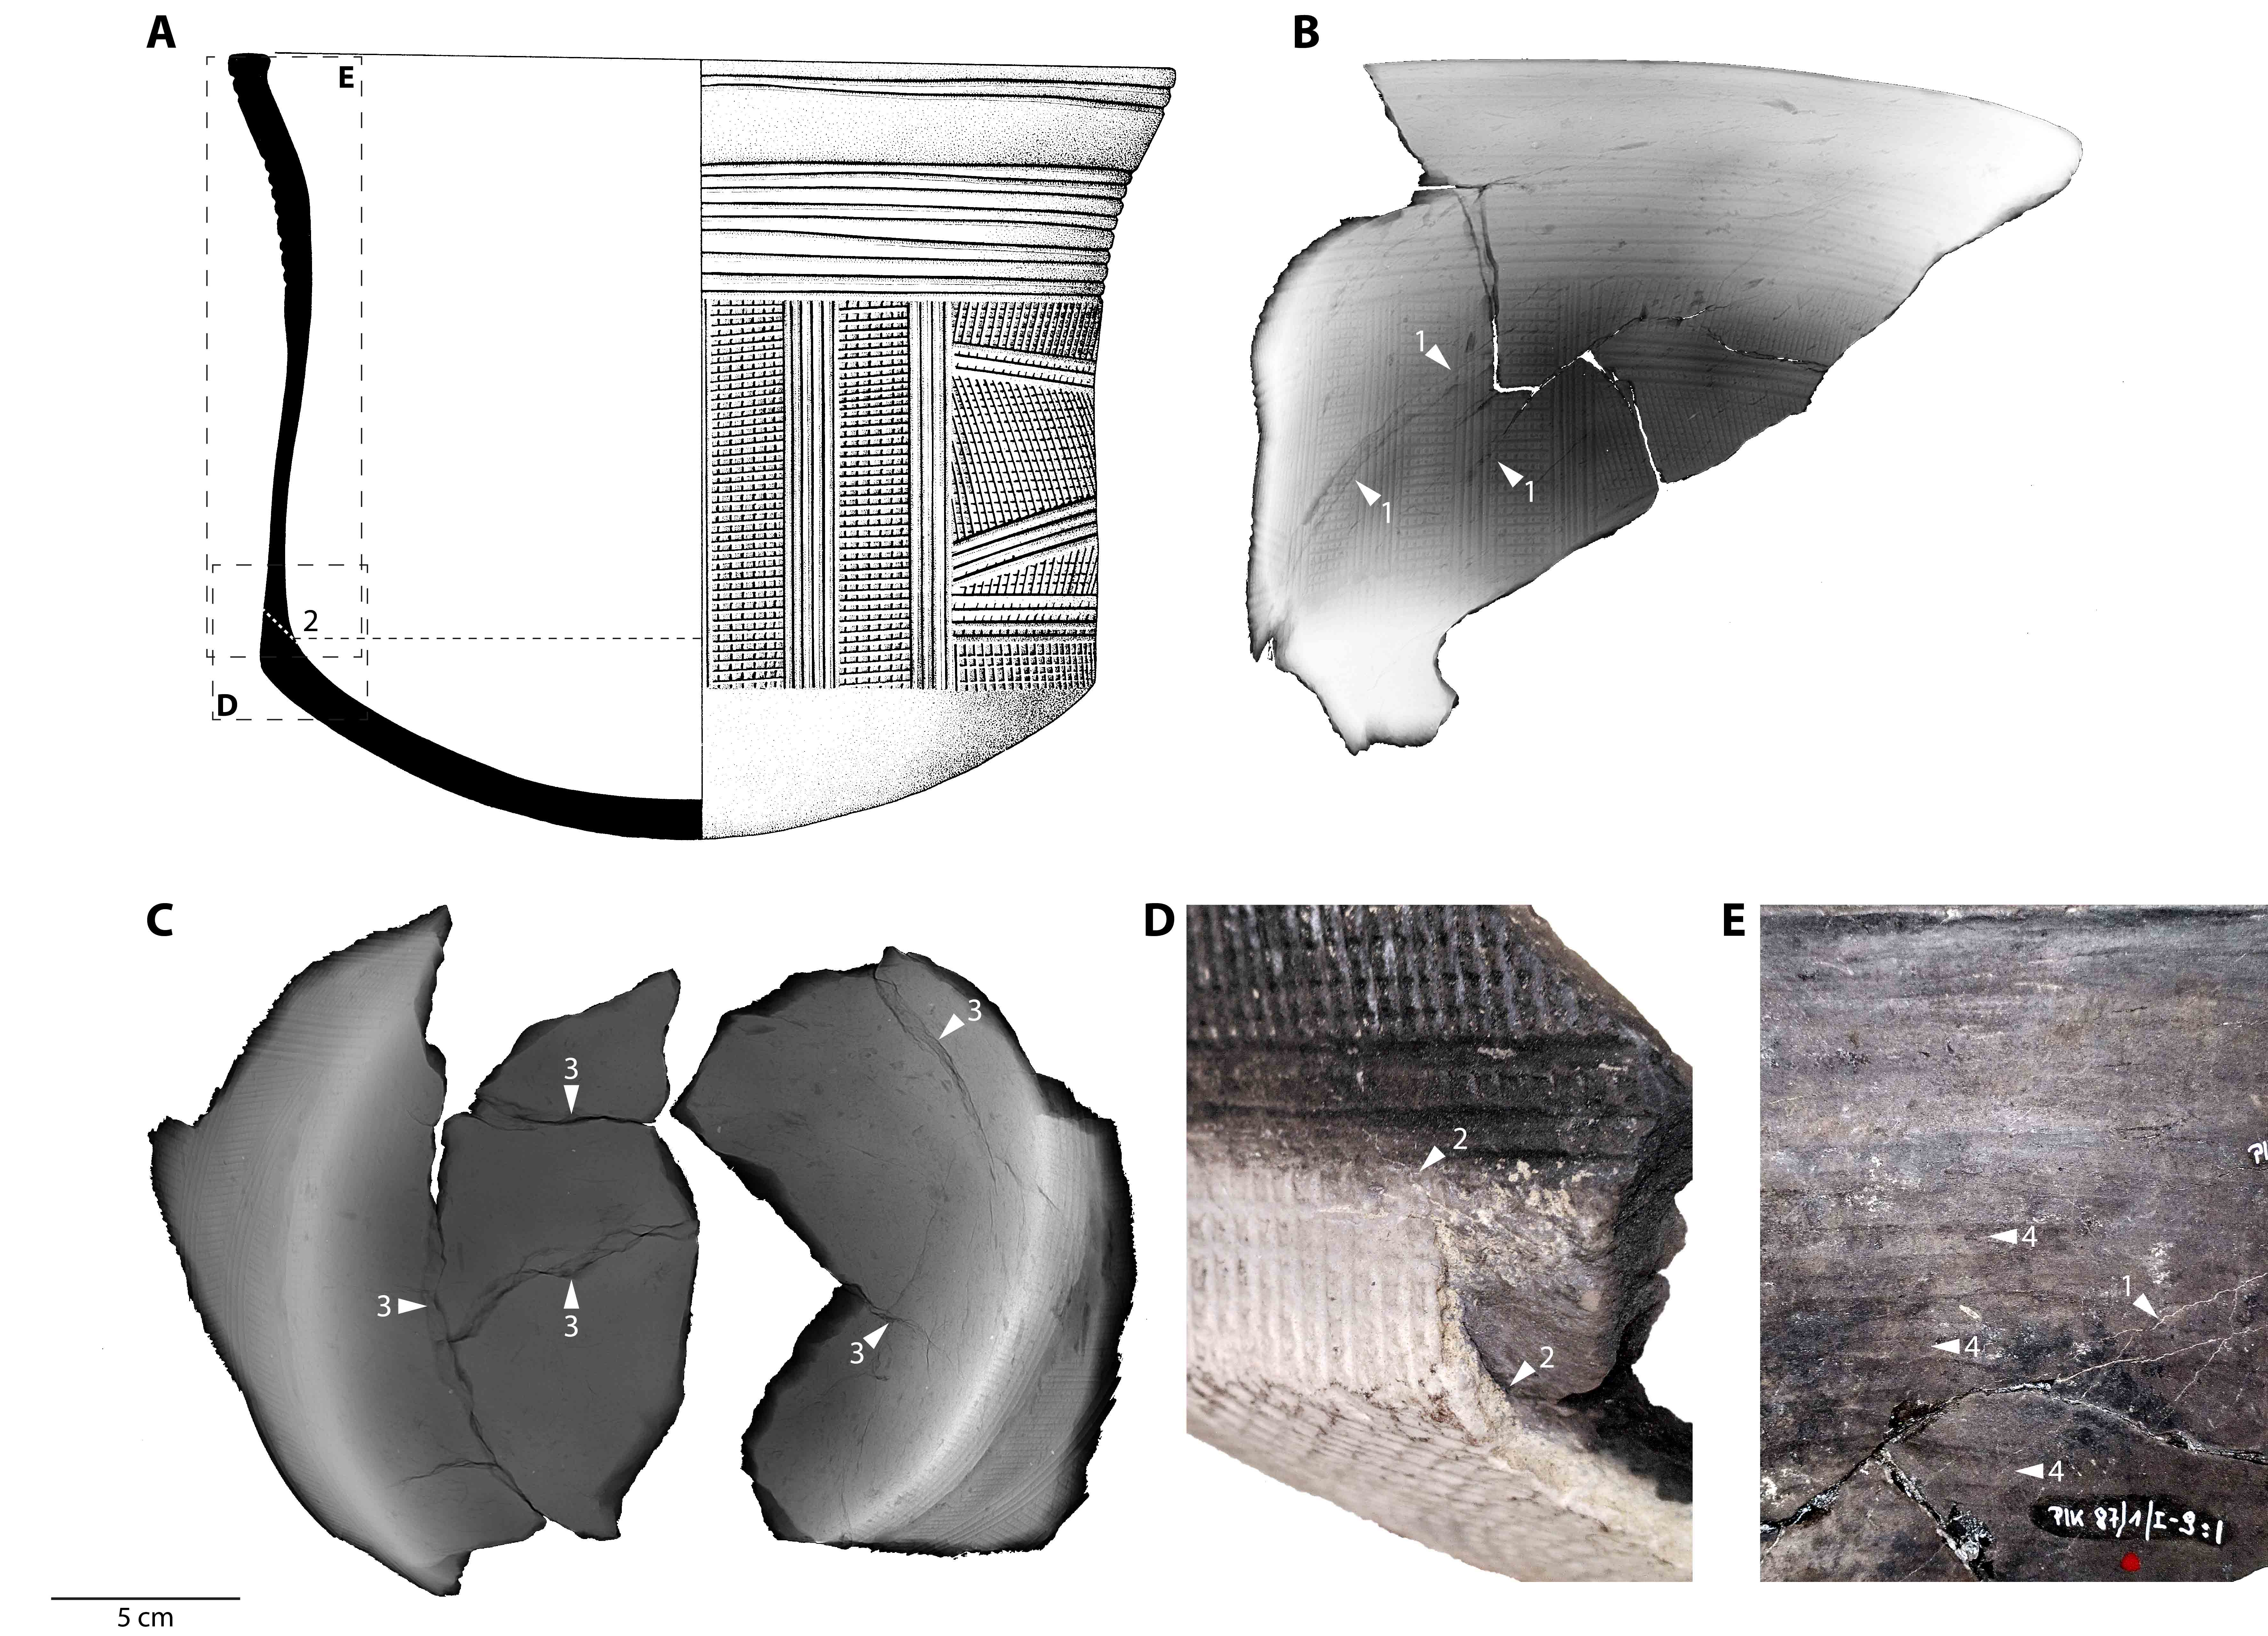
\includegraphics[width=\textwidth]{mt_PIK87-1-8_1-01.jpg}
		\captionof{figure}{Technical observations on PIK 87/1-8:1: (1) helical fissures and breaks; (2) joint between the wall and base; (3) radial and concentric fissures and breaks in the base; (4) horizontal polishing facets on the inside; no illustrations availanble: wall-parallel lamination in the breaks and paddle marks on the exterior of the base. (B: X-ray from lateral; C: X-Ray from inferior; D: Detail of carination; E: View of interior surface) \label{fig:PIK87_1-8_1_macrotraces}}
	\end{minipage}
	\noindent\begin{minipage}{\textwidth}
		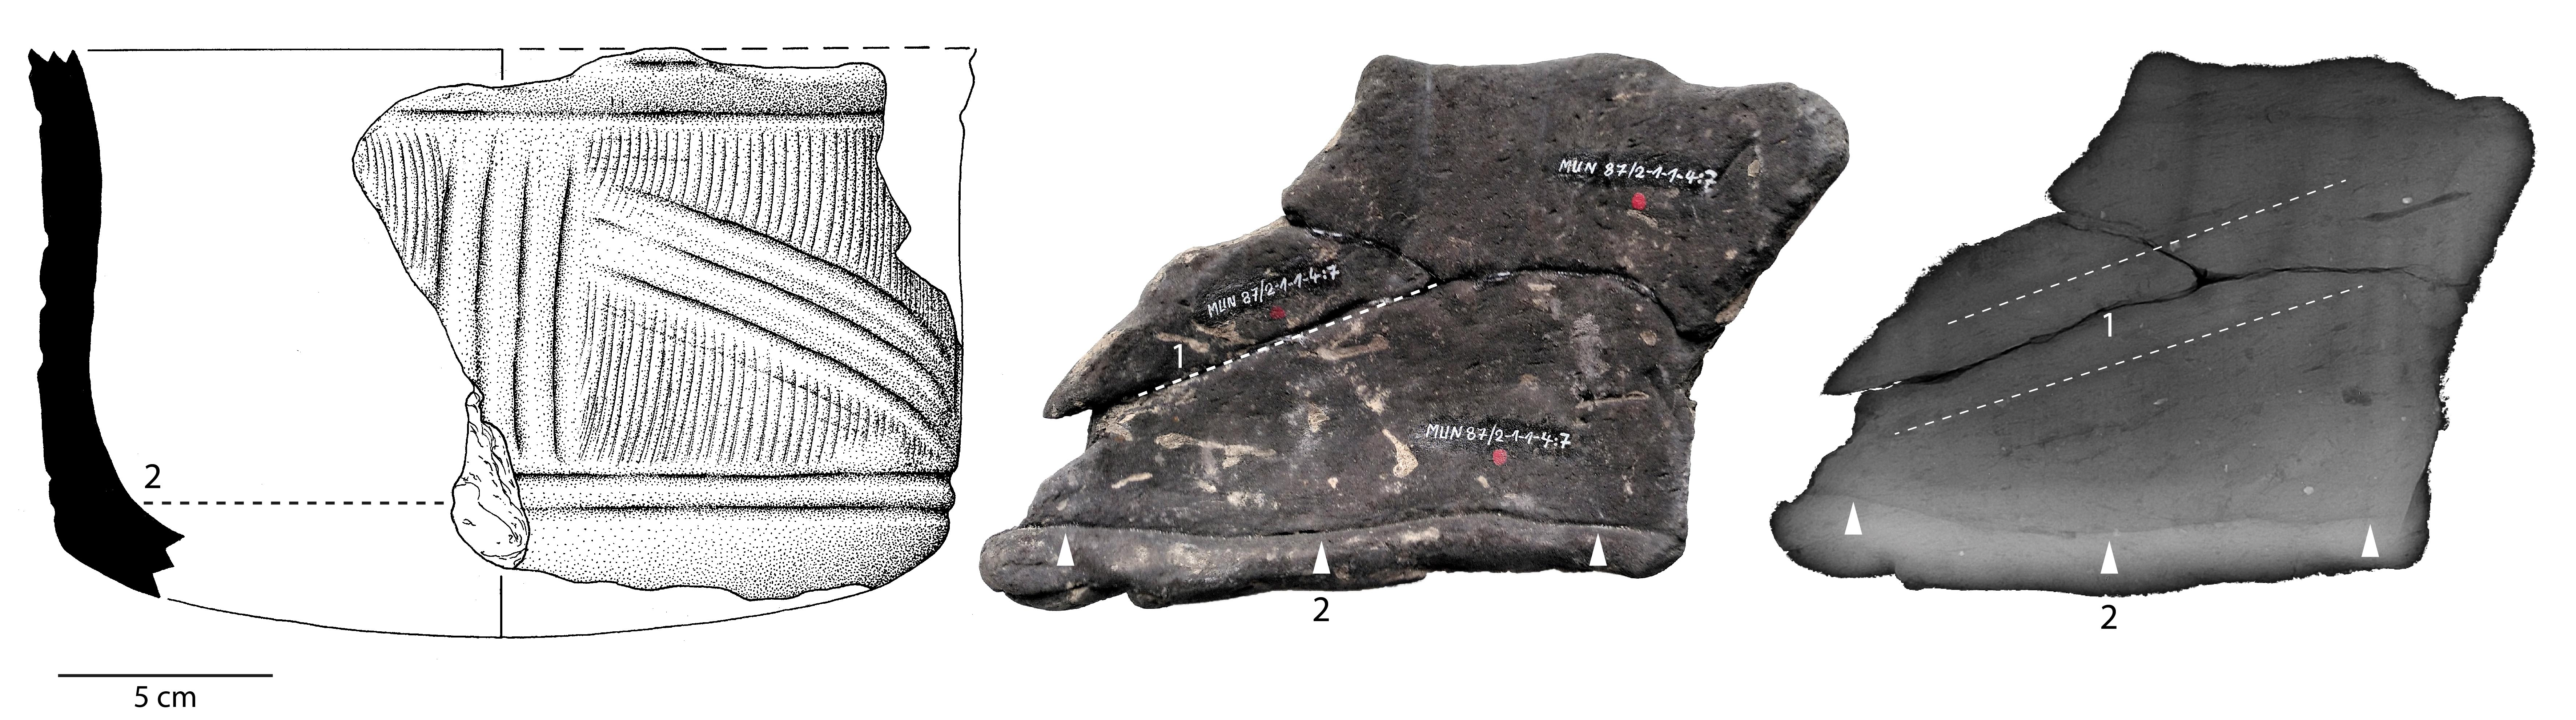
\includegraphics[width=\textwidth]{mt_MUN87_211-4_7-01.jpg}
		\captionof{figure}{Technical observations on MUN~87/2-1-1-4:7: (1) helical fissures and breaks; (2) horizontal joint connecting the wall and the base (B: View from posterior; C: X-ray from posterior).\label{fig:MUN87_211-4_7_macrotraces}}
	\end{minipage}
\end{figure*}

\begin{figure*}[!tb]
	\includegraphics[width=\textwidth]{mt_MUN87_211-5_2-01.jpg}
	\caption{Technical observations on MUN~87/2-1-1-5:2: (1) horizontal polishing facets; (2) helical fissures and breaks; (3) vertical lamination of the wall; (4) concentric break; (5) radial fissures and cracks; (6) thickening of the base. (A: X-ray from superior; B: View from posterior; D: View from lateral; E: View from inferior; F: Detail of breakage)}
	\label{fig:MUN87_211-5_2_macrotraces}
\end{figure*}

\begin{figure*}[p]
	\centering
	\includegraphics[width=.8\textwidth]{mt_MUN87_211-8_1-01.jpg}
	\caption{Technical observations on MUN~87/2-1-1-8:1: (1) single vertical fissure and crack in the wall; (2) horizontal compression folds near the base; (3) radial fissures in the base; (4) thickening on the outside at the base. (A: X-ray from superior; B: View from superior; D: Detail of interior surface; E: Detail of transition of wall to base; F: Detail of interior surface at transition of wall to base)}
	\label{fig:MUN87_211-8_1_macrotraces}
\end{figure*}

\begin{figure*}[p]
	\centering
	\includegraphics[width=.8\textwidth]{mt_MUN87_211-8_2-01.jpg}
	\caption{Technical observations on MUN~87/2-1-1-8:2: (1) single vertical fissure and crack in the wall; (2) helical fissures; (3) concentric fissures; (4) thinning of the base and paddle marks. (A: X-ray from superior; B: View from lateral; C: View from inferior; D: View from superior; E: Detail from lateral; F: Detail of the interior surface)}
	\label{fig:MUN87_211-8_2_macrotraces}
\end{figure*}

The primary shaping technique of Pikunda-Munda potters has been identified based on macro-traces and radiograph features. Common among Pikunda-Munda vessels, often wide-mouthed bowls with parallel or concave sides, flared rims, and round bases, are helical fissures, cracks, or breaks (Fig.~\ref{fig:PIK87_1-8_1_macrotraces}, \ref{fig:MUN87_211-4_7_macrotraces}, \ref{fig:MUN87_211-5_2_macrotraces}, and \ref{fig:MUN87_211-8_2_macrotraces}). This feature, usually occurring during the drying stage, indicates an upward, rotating movement the potter applies during the primary shaping stage. A similar technique was documented at the potters' village of Ikenge on the Ruki river \citep[Fig.~\ref{fig:map}; ][]{Eggert.1980c}. Another common feature is wall-parallel 'lamination', usually visible on the breaks (Fig.~\ref{fig:MUN87_211-5_2_macrotraces}) or as flaking of the surface. These two features indicate a drawing technique to be applied by Pikunda-Munda potters to shape the upper parts of the vessels.

Nearly all vessels studied showed some signs that their upper parts and bases were pre-shaped separately. While all features of the upper parts of the vessels are strikingly similar, indicating that the potters performed similar actions and motions to shape these parts, two modes of constructing the bases were observed. The most widespread configuration of features is radial as well as concentric fissures, cracks or breaks in the base (Fig.~\ref{fig:MUN87_211-5_2_macrotraces}, \ref{fig:MUN87_211-8_1_macrotraces}, and \ref{fig:MUN87_211-8_2_macrotraces}). These are regularly coupled with patchy differences in the densities of the base, as observed in the radiographs. This set of co-occurring features is distinct from the features observed at the upper parts. The current working hypothesis is that these features are the remains of additional clay used to 'close' the rough-out. After adding clay, the base was then shaped using pounding and paddling, similar to what \citet{Eggert.1980c} documented at Ikenge.

A second, slightly different mode is attested for in two vessels (Fig.~\ref{fig:PIK87_1-8_1_macrotraces}--\ref{fig:MUN87_211-4_7_macrotraces}) and characterized by a visible joint between the wall and the base, right at the carination. In one particular case (Fig.~\ref{fig:PIK87_1-8_1_macrotraces}), the base overlaps the wall, with a small part of the decoration of the upper parts even being covered. This indicates that the upper part must have been roughed-out, shaped, and already decorated before the base, presumably pre-shaped separately, was attached. Thus, this second mode combines the drawing of a ring technique with a slab bottom.

That the initial rough-out was shaped by drawing of a ring \citep[cf.][]{LivingstoneSmith.2010a}, which is a different technique from the pierced lumps observed at Ikenge \citep{Eggert.1980c}, can be deduced from singular vertical fissures and cracks in some vessels (Fig.~\ref{fig:MUN87_211-8_1_macrotraces}--\ref{fig:MUN87_211-8_2_macrotraces}). This feature is interpreted as a remnant of the construction of the initial ring.

The configuration of features constituting core stages of the \textit{chaîne opératoire} of Pikunda-Munda potters consists of helical fissures, cracks of breaks in the upper part, lamination visible in the breaks, and either the addition of clay to close the base, involving usage of pestles and paddles, or slab bottoms. 

\begin{figure*}[p]
	\noindent\begin{minipage}[b]{.48\textwidth}
	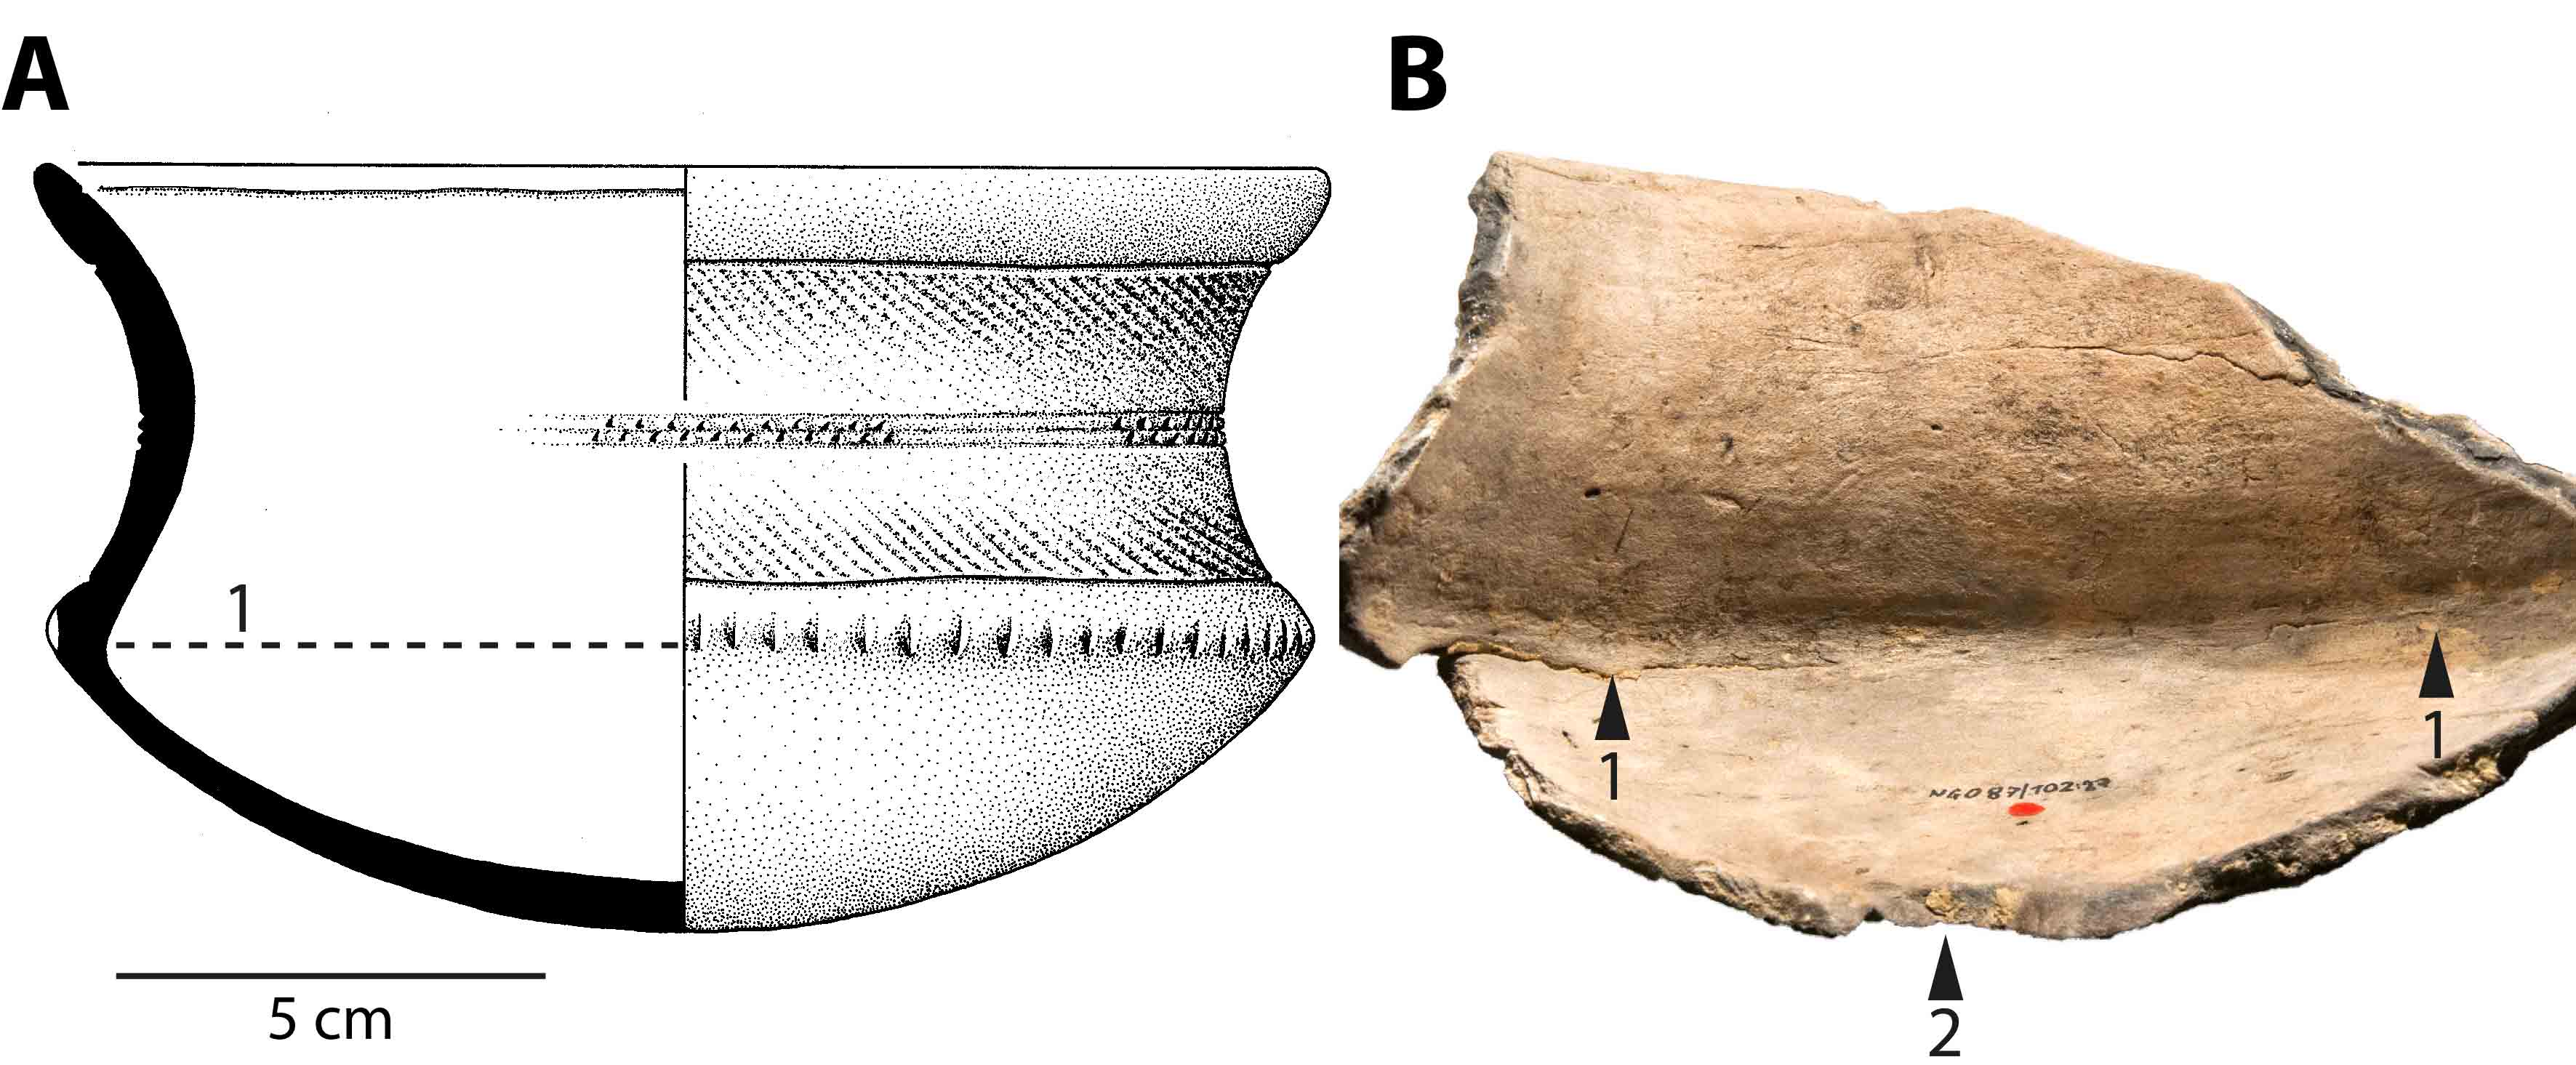
\includegraphics[width=\textwidth]{mt_NGO87-102_27-01.jpg}
	\captionof{figure}{Technical observations on NGO~87/102:27: (1) horizontal fissures and cracks indicating joining of two parts; (2) concentric break of the base. (B: View of the interior surface)\label{fig:NGO87_102_27_macrotraces}}
	\vspace{1.5em}
	\captionof{figure}{Technical observations on NGO~87/102:28--29: (1) thickening of the wall; (2) horizontal scraping; (3) horizontal break, indicating joining of two pieces; (4) thinning of th wall; (5) pounding marks and thinning of the wall. (A: Detail of the interior surface at the upper part)\label{fig:NGO87_102_28-29_macrotraces}}
	\end{minipage}\hfill
	\noindent\begin{minipage}[b]{.48\textwidth}
	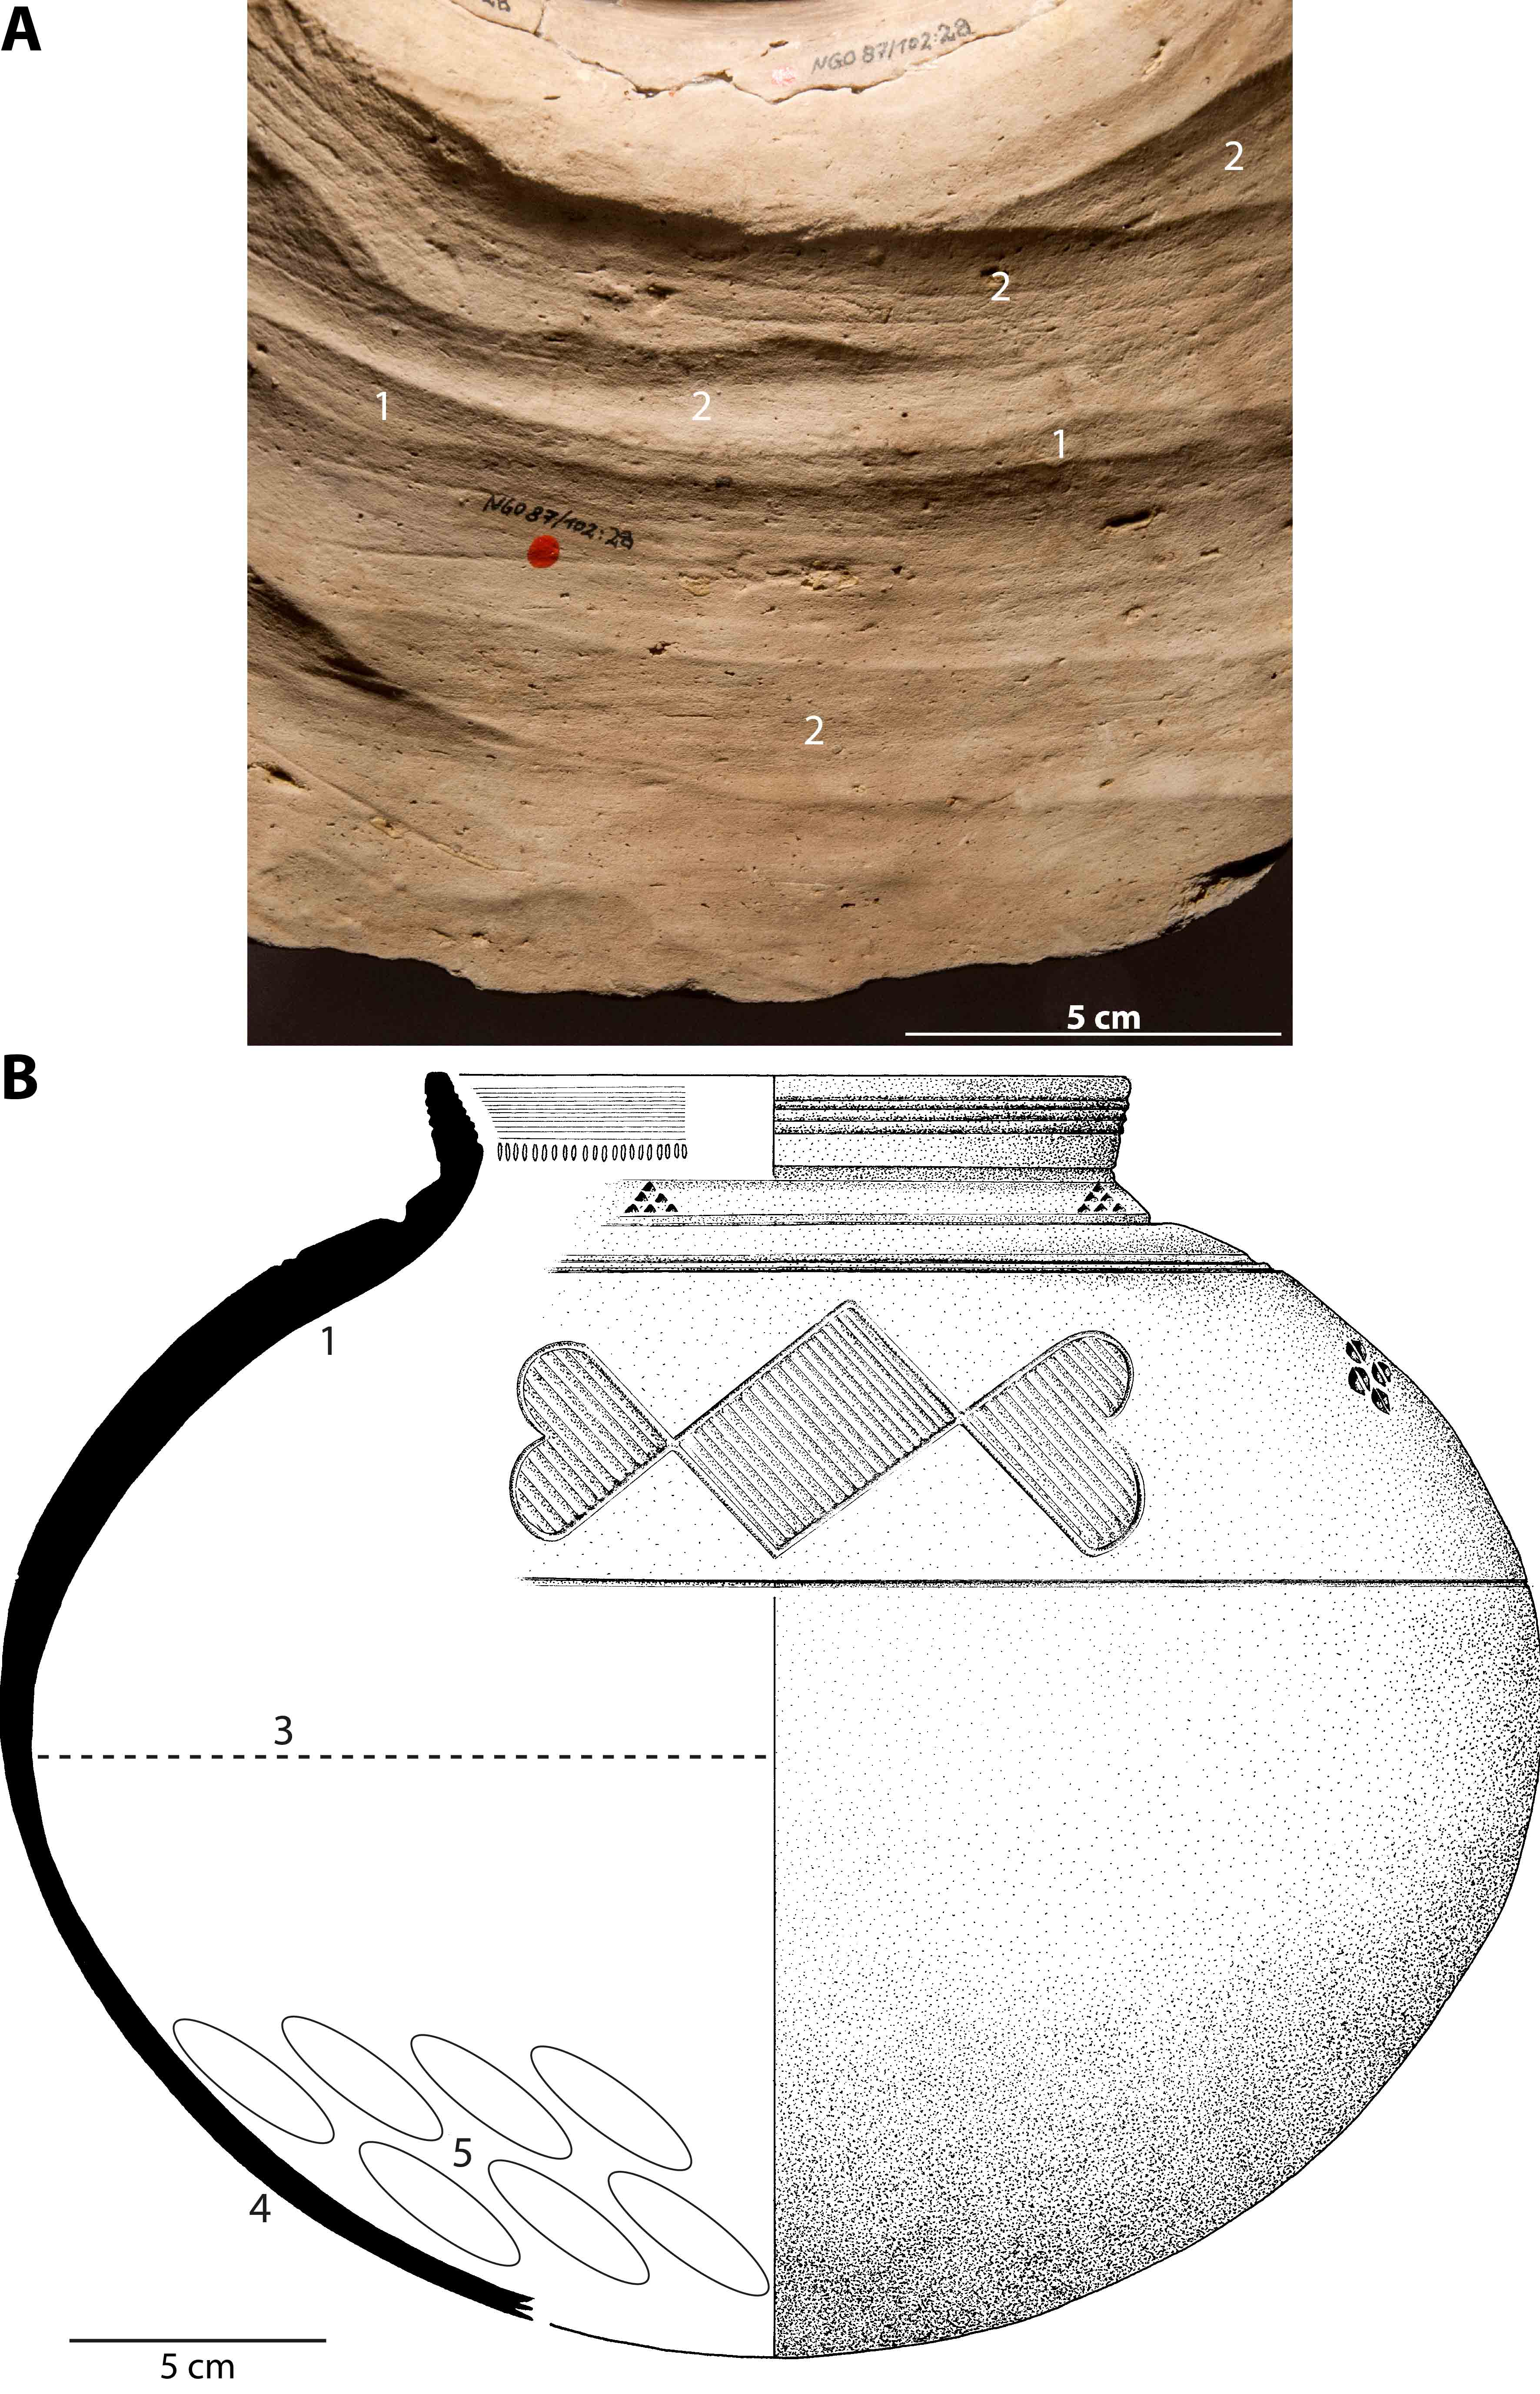
\includegraphics[width=\textwidth]{mt_NGO87-102_28-29-01.jpg}
	\end{minipage}
\end{figure*}

\begin{figure*}[p]
	\noindent\begin{minipage}[t]{.65\textwidth}
		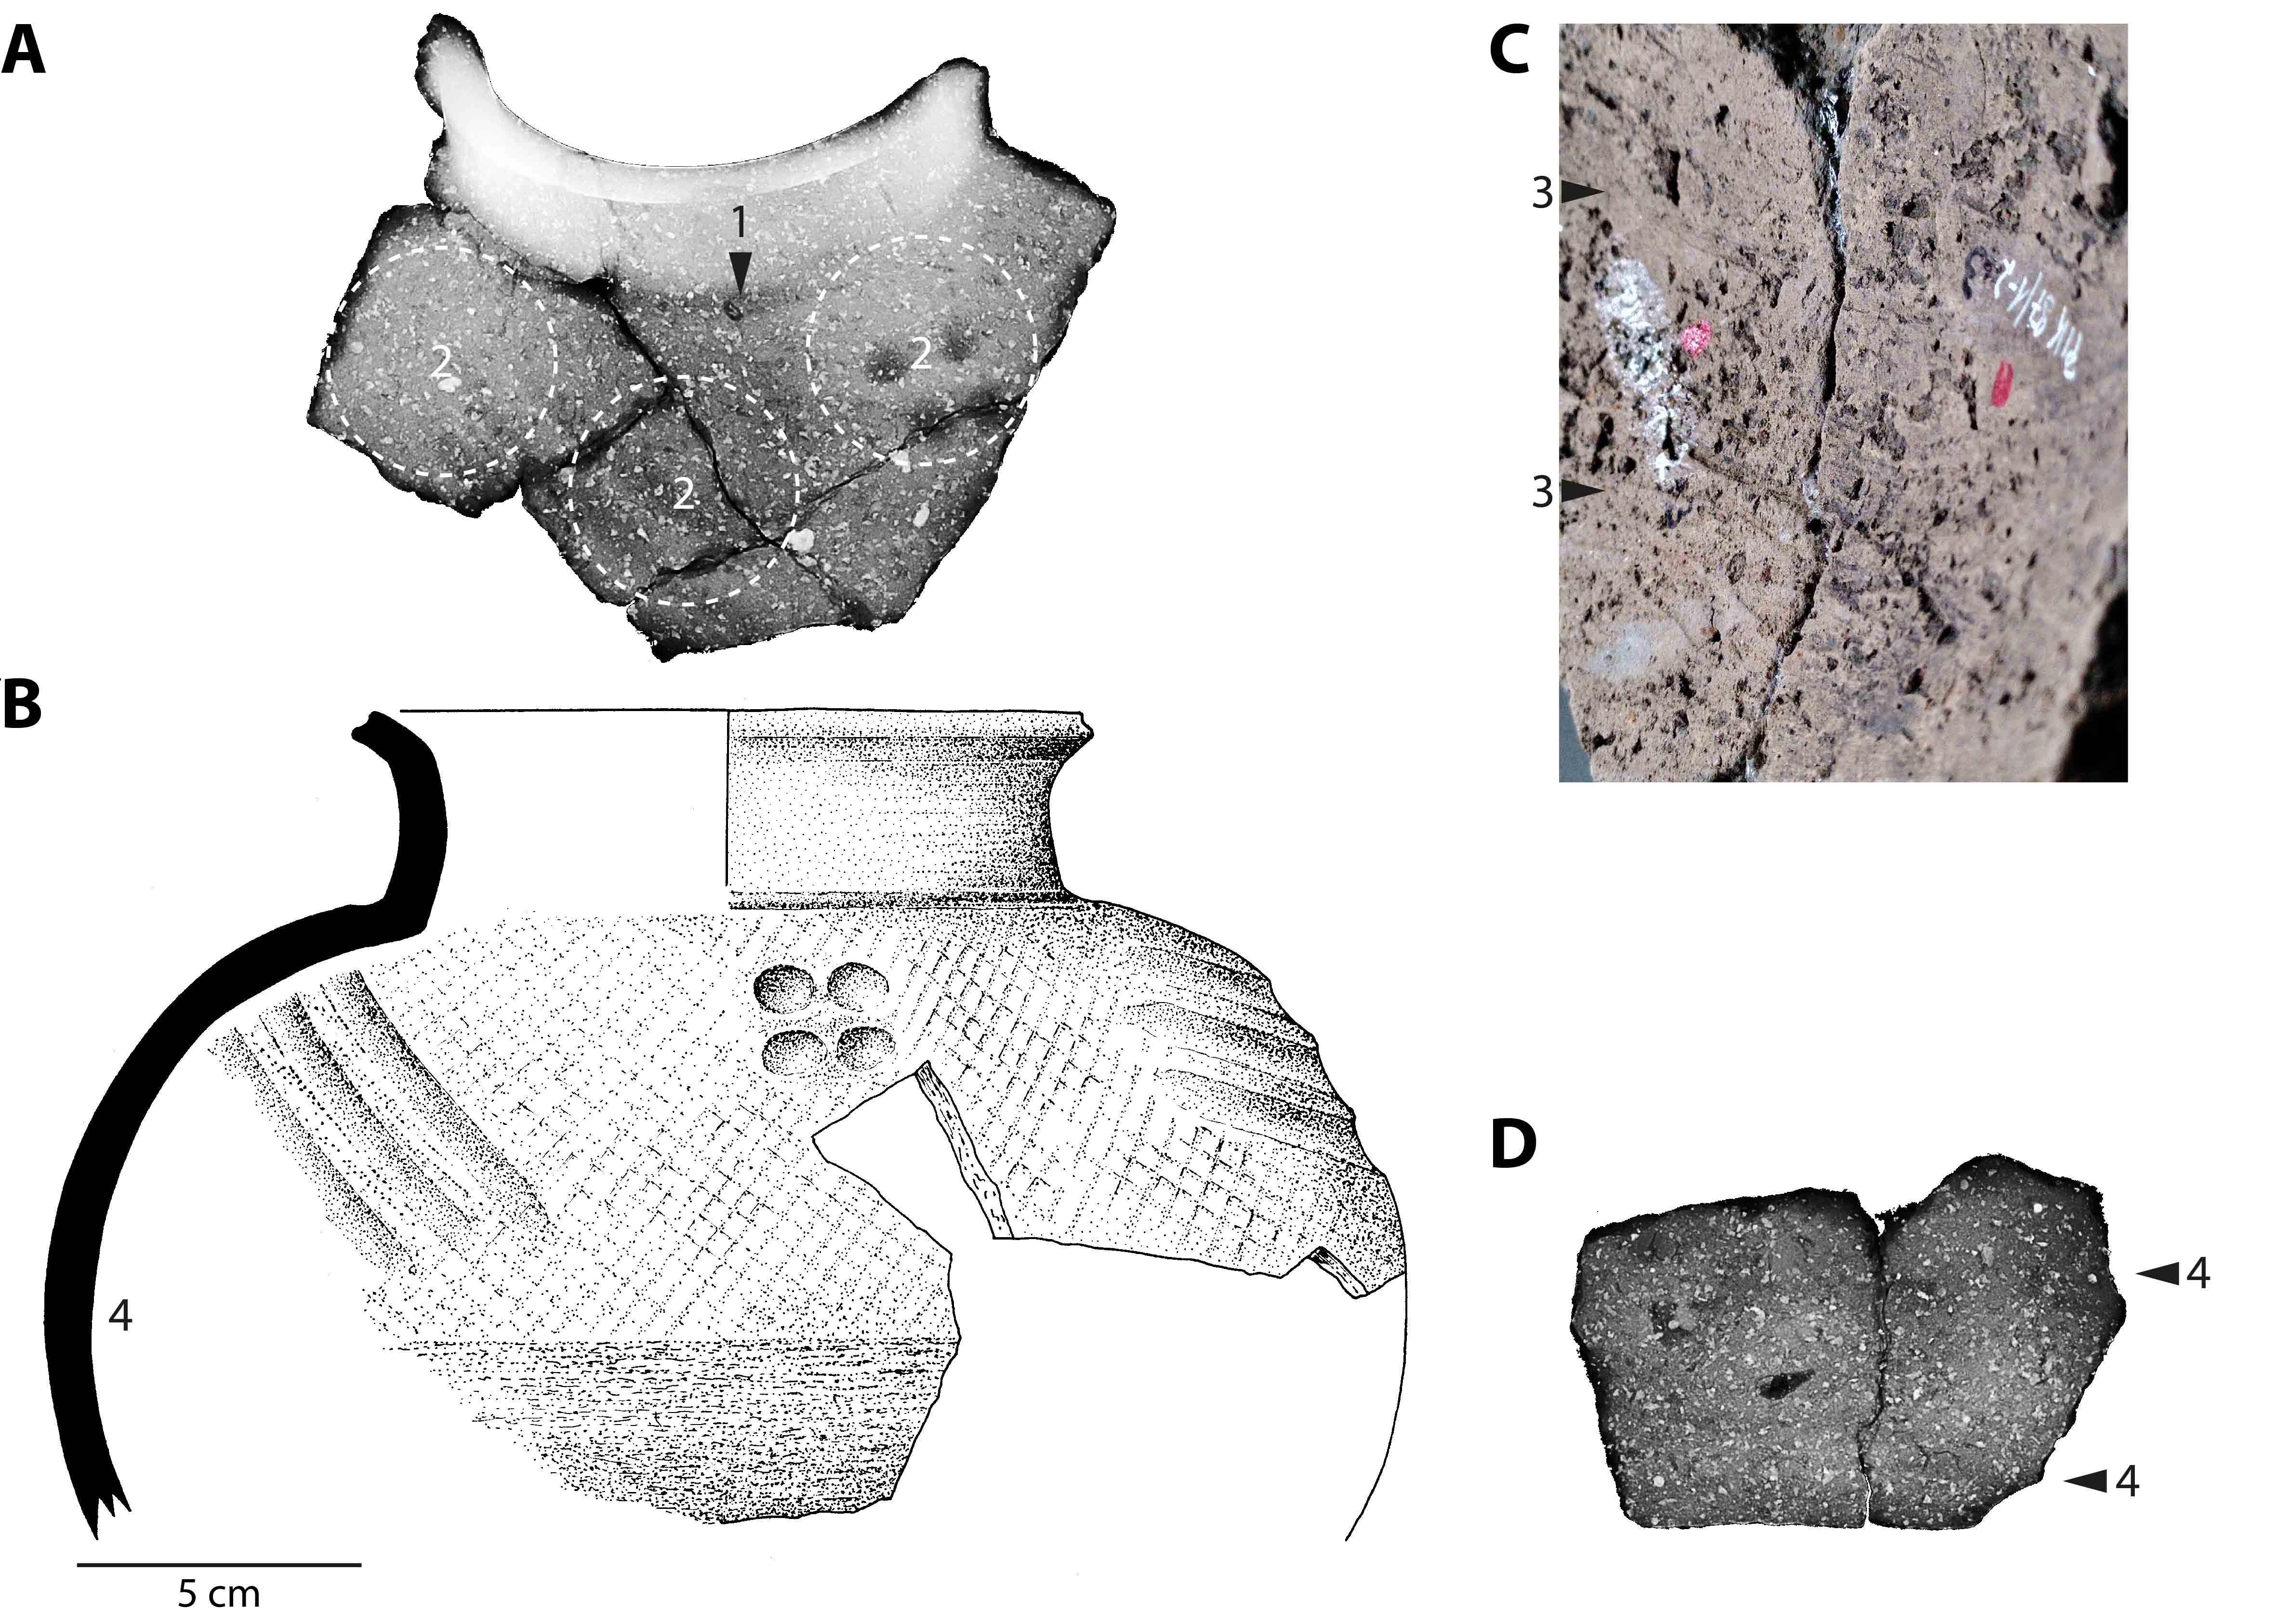
\includegraphics[width=\textwidth]{mt_PIK87-1-2_3-01.jpg}
		\captionof{figure}{Technical observations on PIK~87/1-2:3: (1) reduced density indicating join for the rim to the neck; (2) patches of higher and lower density; (3) fine scraping on the interior surfaces; (4) horizontally organized changes in density indicating remants of coils. (A: X-ray from superior; C: Detail of interior surface from D; D: X-ray from lateral)\label{fig:PIK87_1-2_3_macrotraces}}
	\end{minipage}\hfill
	\noindent\begin{minipage}[t]{.32\textwidth}
		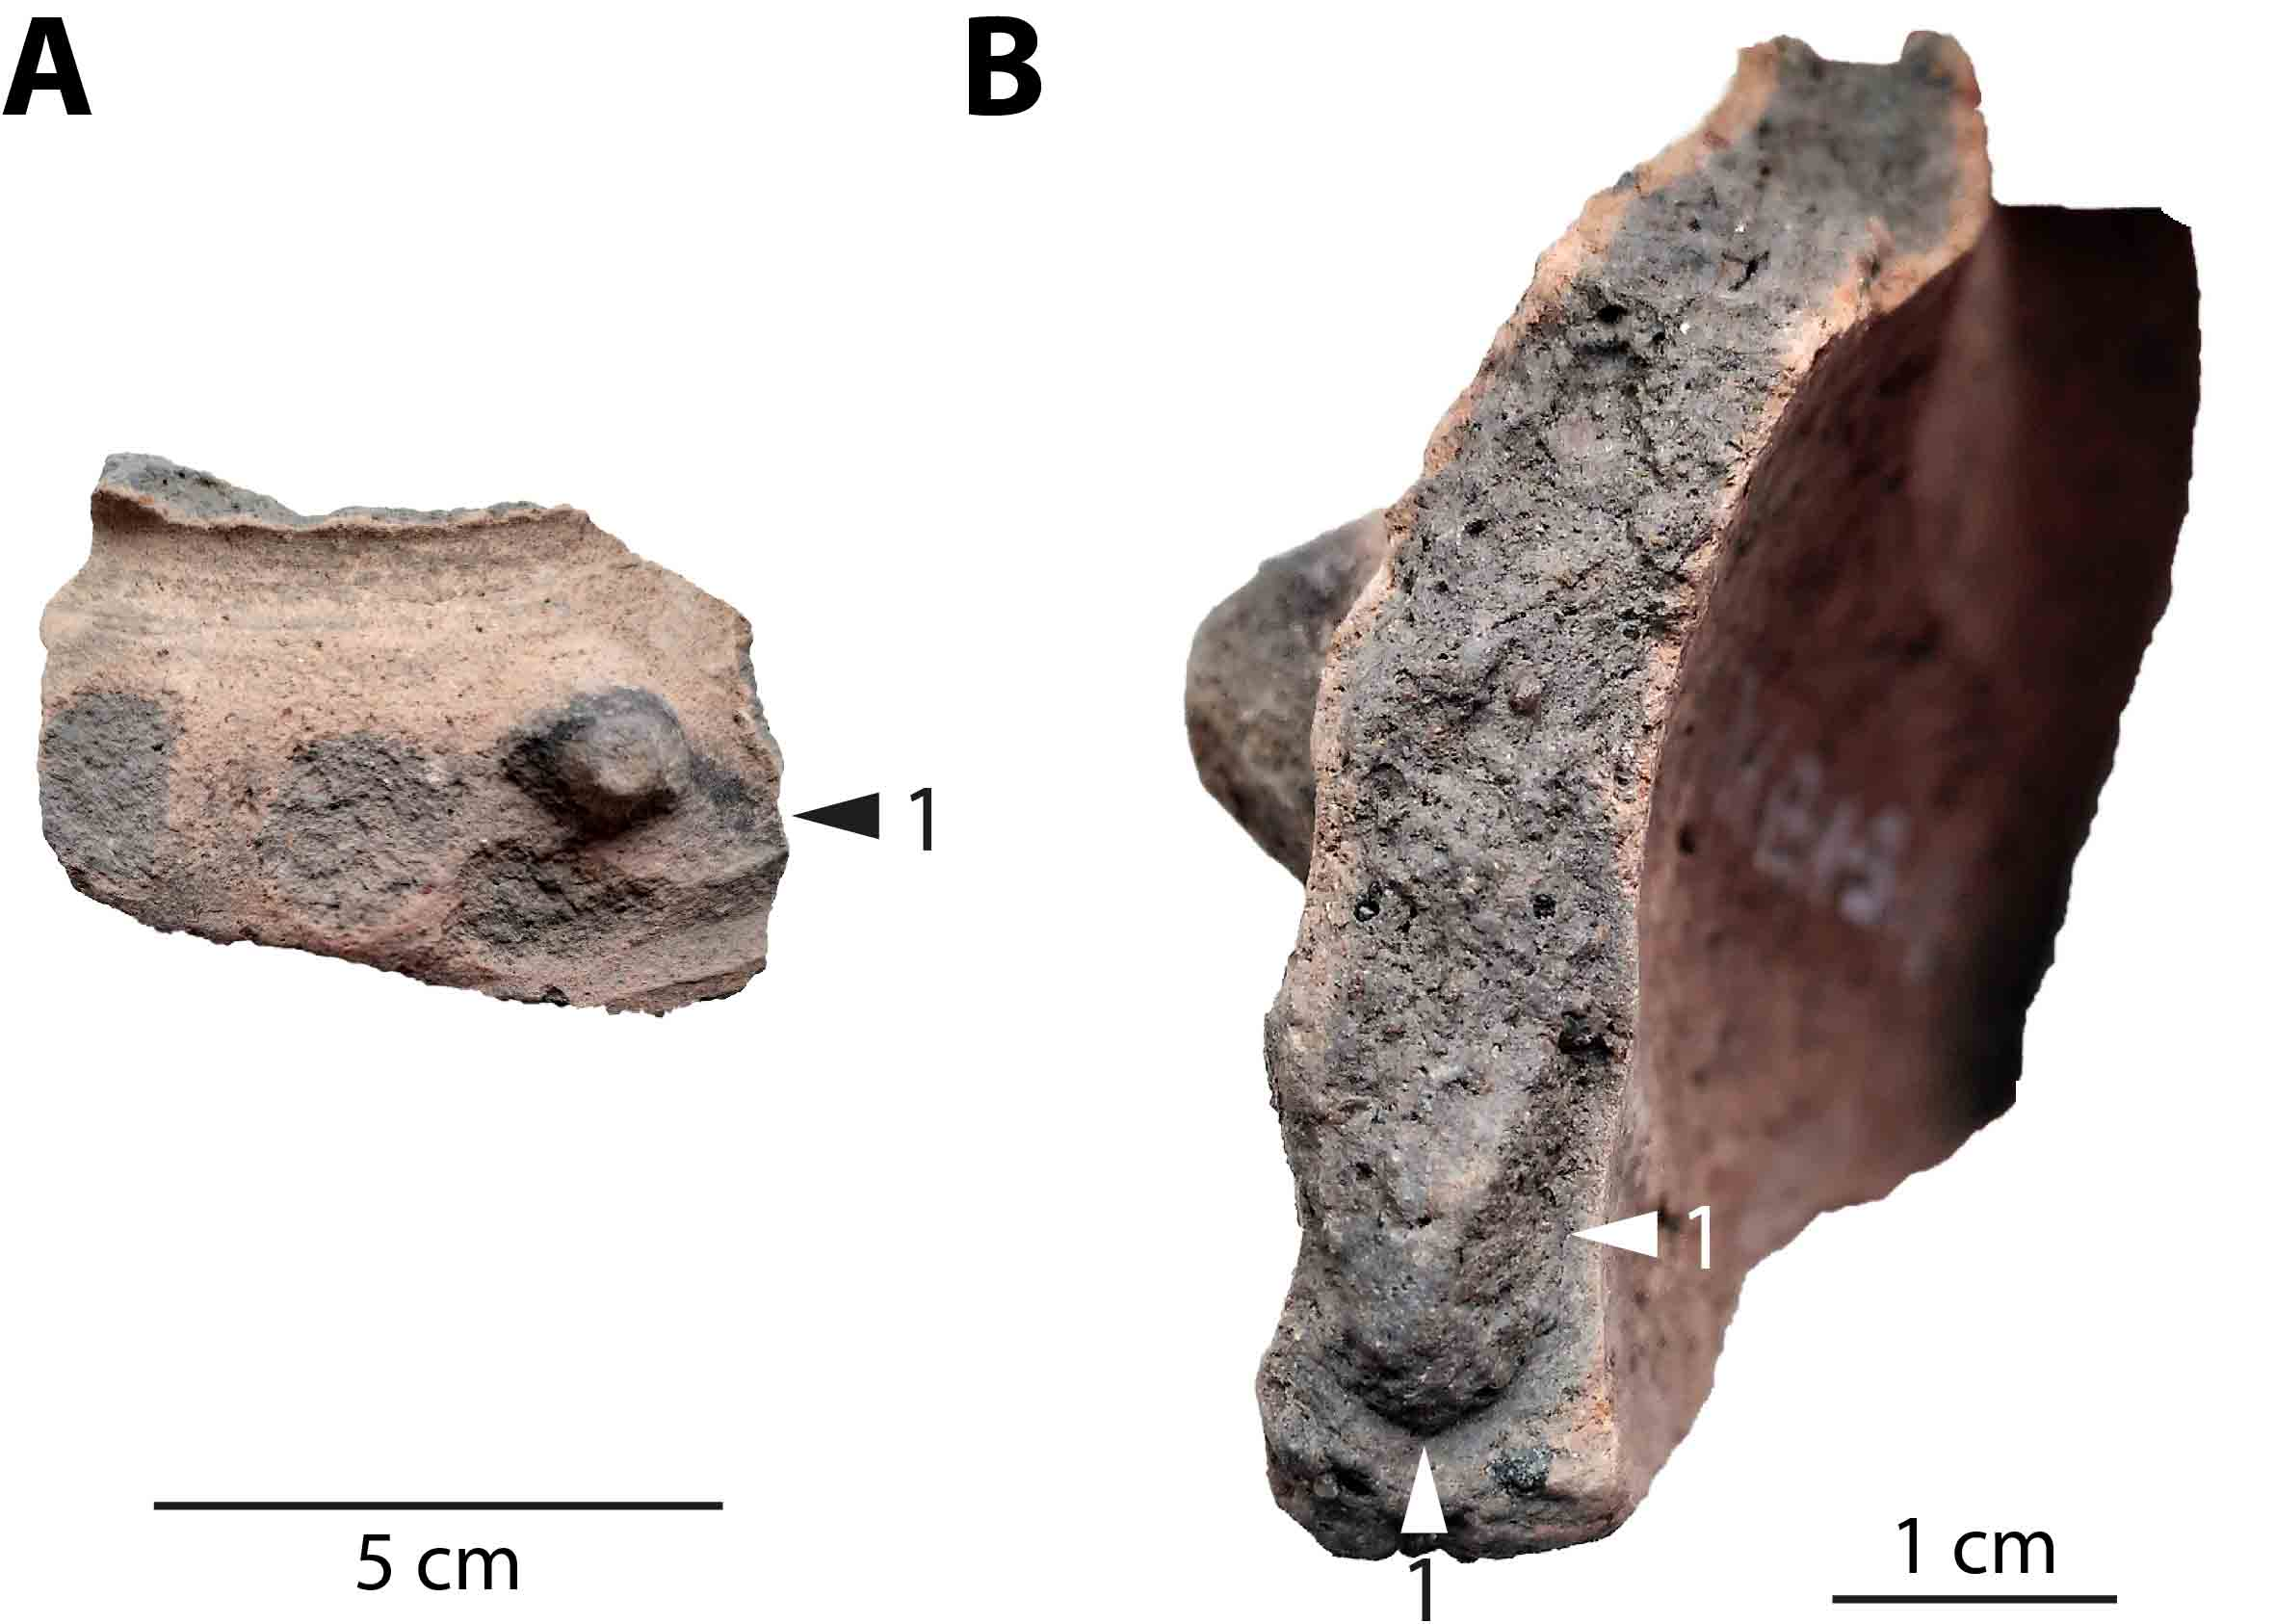
\includegraphics[width=\textwidth]{mt_PIK87-1-3_-01.jpg}
		\captionof{figure}{Technical observations on PIK~87/1-3:? (1) remnants of a coil vissible in the break. (A: View from lateral; B: Detail of breakage) \label{fig:PIK87_1_macrotraces}}
	\end{minipage}
\end{figure*}

\begin{figure*}[!tb]
	\centering
	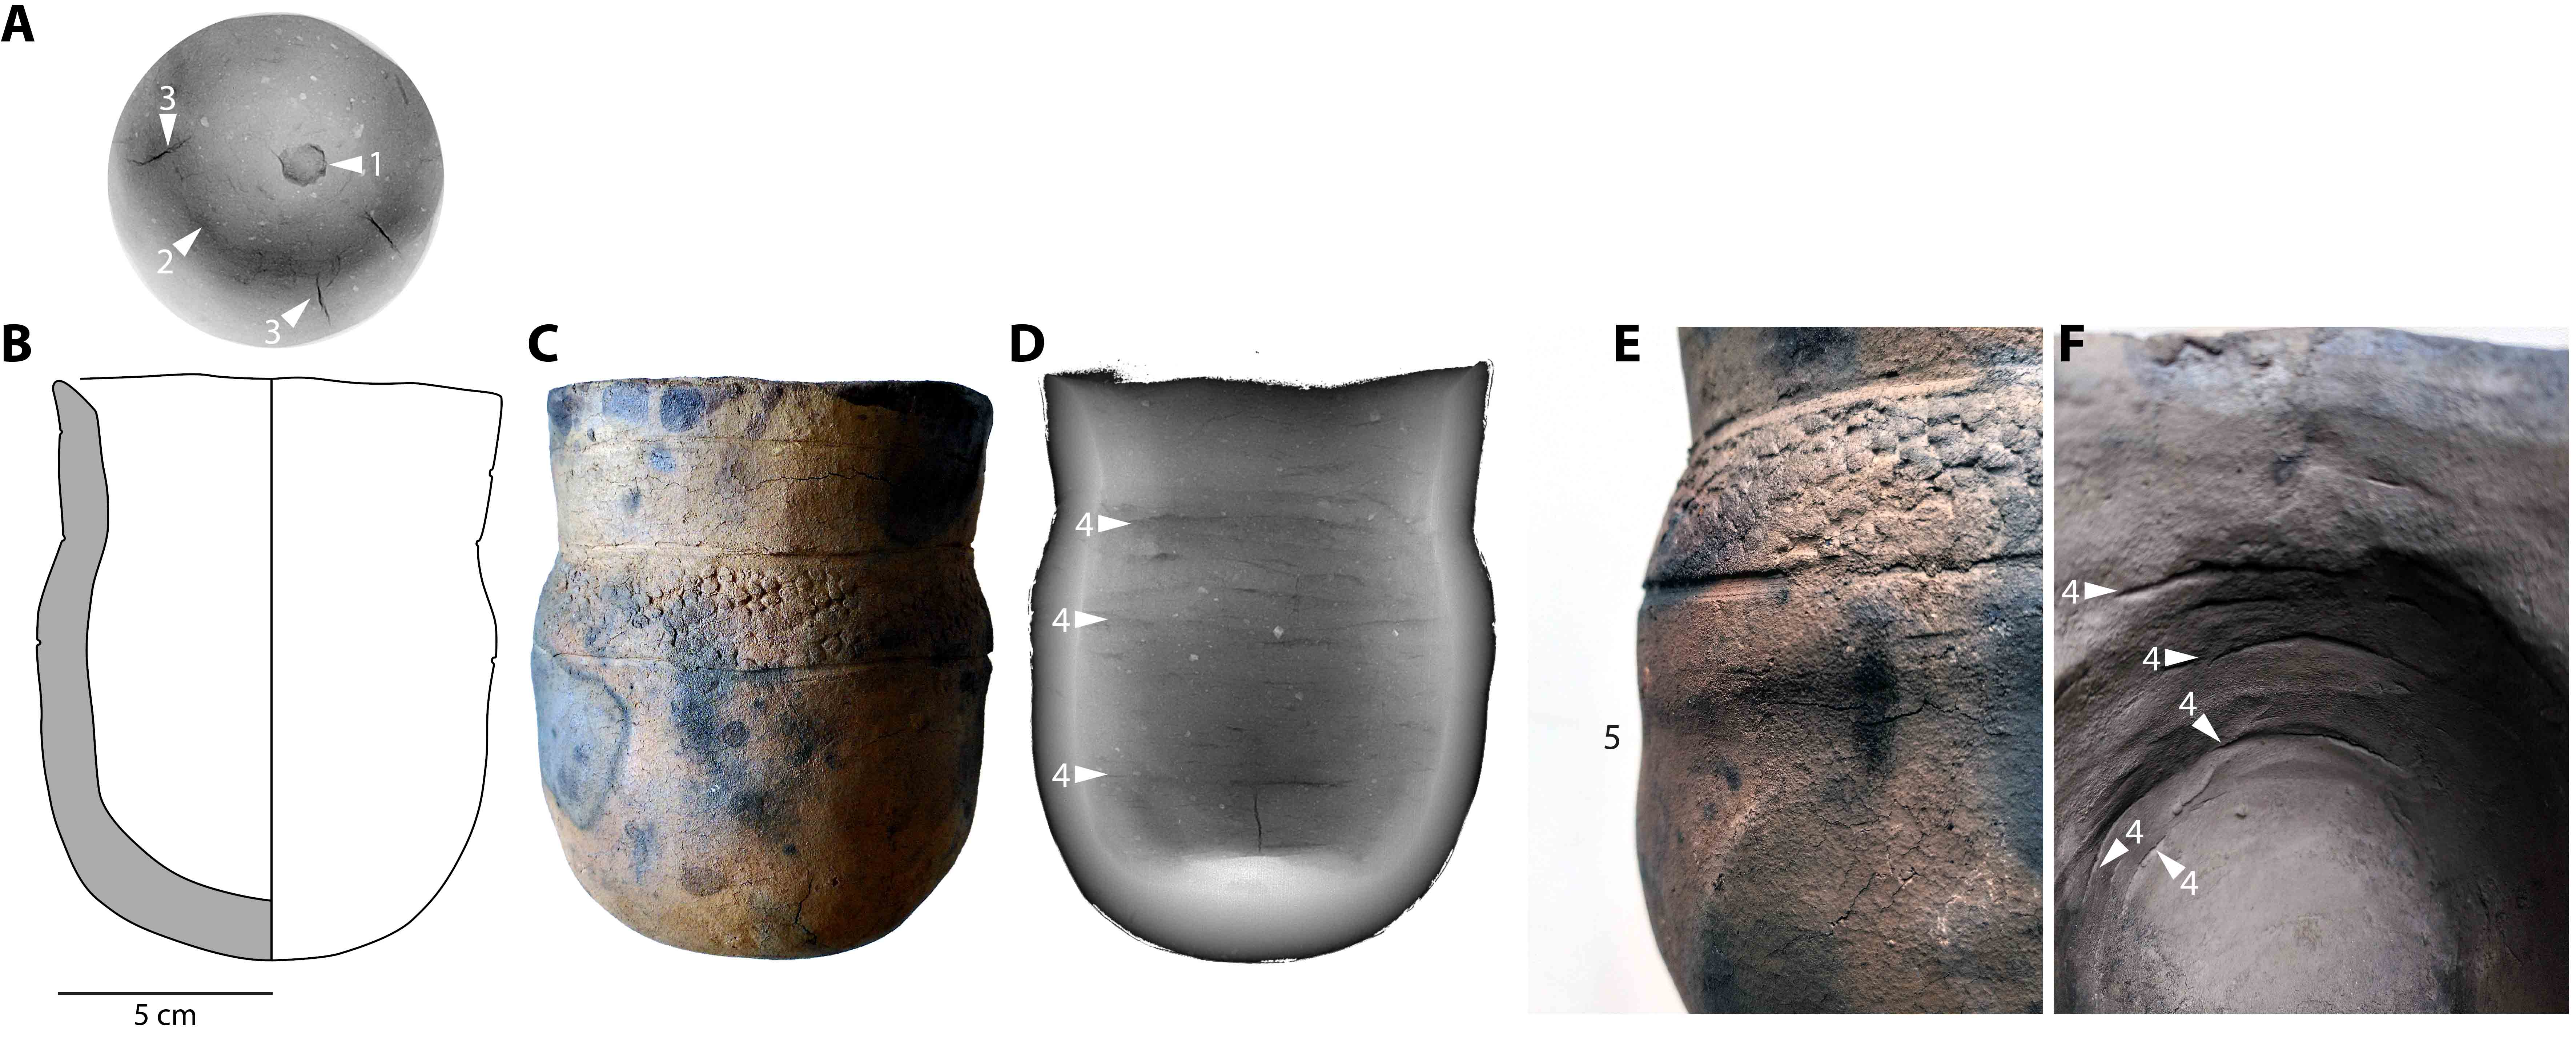
\includegraphics[width=\textwidth]{mt_PIK87-501_2-01.jpg}
	\caption{Technical observations on PIK~87/501:2: (1) remnant of the removed fruit seed used as onset of the coiling; (2) concentric fissures; (3) radial cracks; (4) gaps between coils; (5) horizontally organized variations of the exterior surface of the vessel. (A: X-ray from superior; C: View from lateral; D: X-ray from lateral; E: Detail of exterior surface; F: Detail of interior surface)}
	\label{fig:PIK87_501_2_macrotraces}
\end{figure*}

\begin{figure*}[p]
	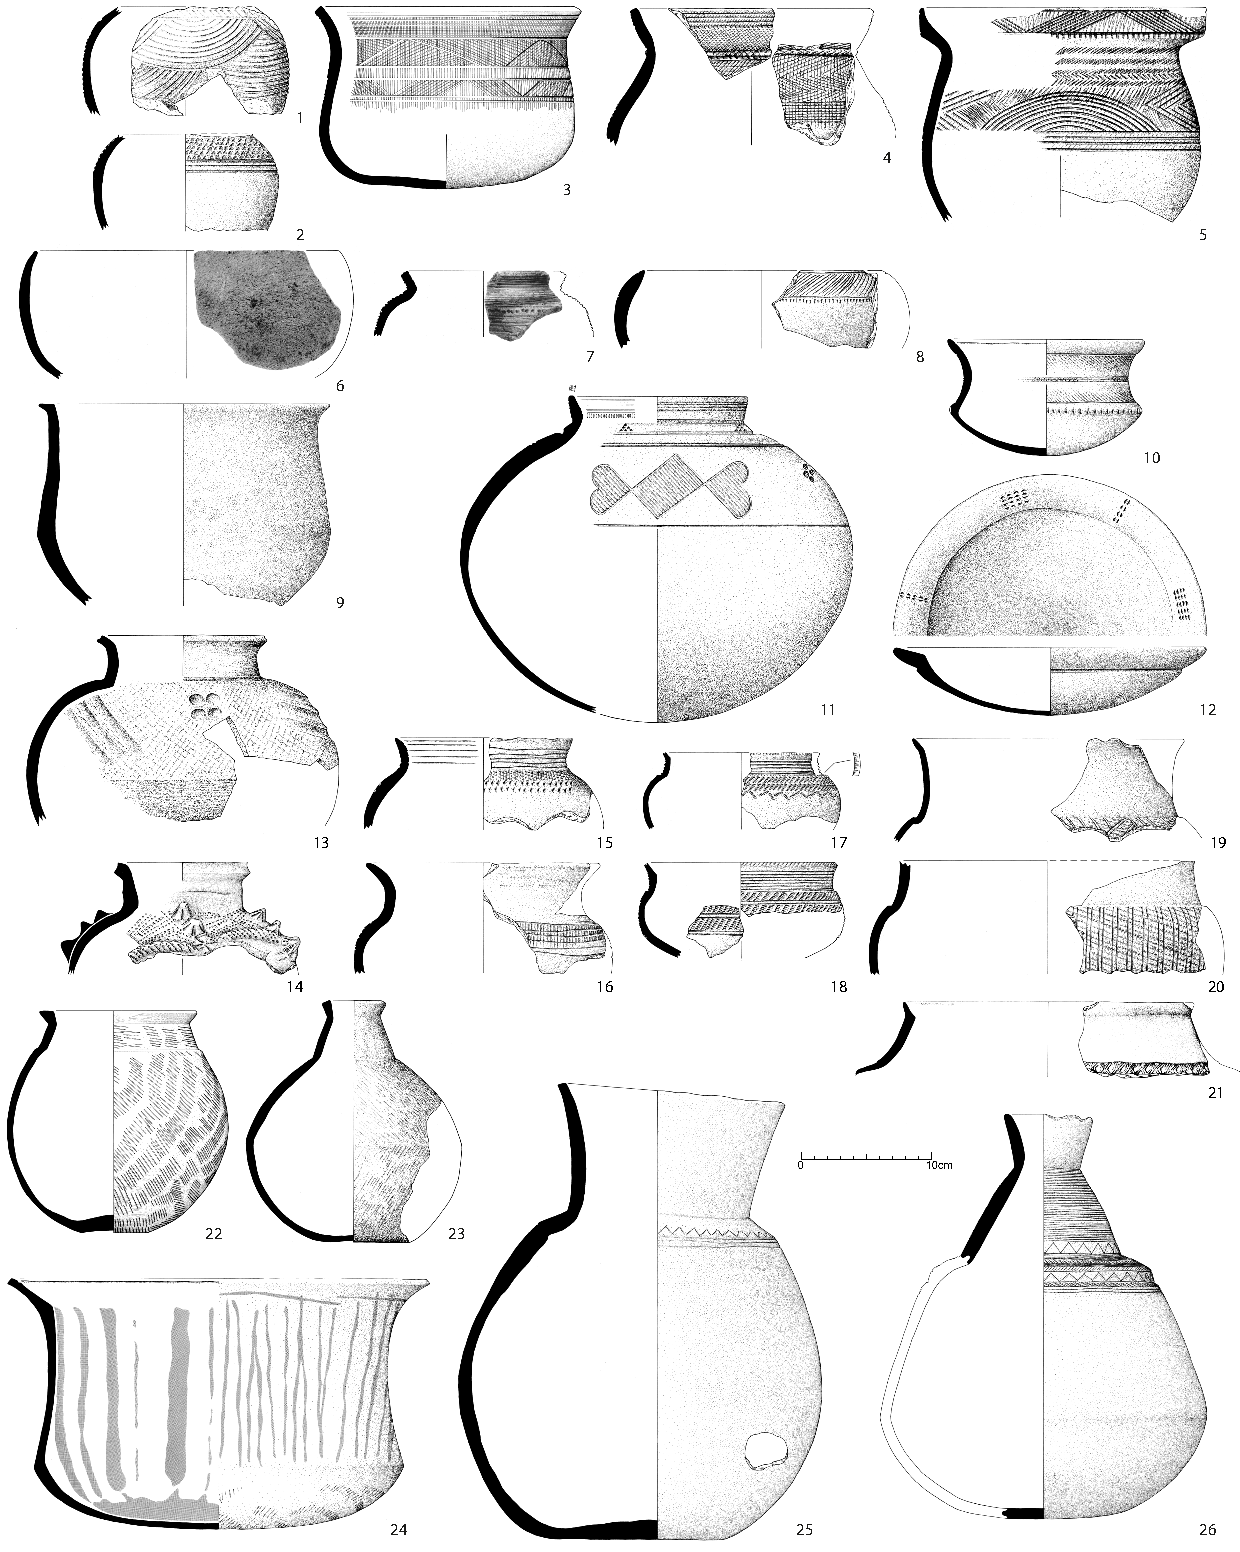
\includegraphics[width=\textwidth]{Fig_Sangha_Typen.pdf}
	\caption{Examples of pottery styles recorded in the Western Congo Basin in general chronological order: 1--2) Imbonga \citep[169--172]{Seidensticker.2021e}; 3--4) Pikunda-Munda (ibid. 114--120); 5) Bokonogo (ibid. 120--123); 6--8) Bobusa (ibid. 162--165); 9) Matoto (ibid. 128--131); 10--12) Ngombe (ibid. 124--128); 13--14) Mandombe (ibid. 145--148); 15--16) Konda (ibid. 148--152); 17--18) Ouesso (ibid. 152--155); 19--20) Pandama (ibid. 155-158); 21) Mbenja (ibid. 158--162); 22--23) Ebambe (ibid. 131--136); 24) Mobaka (ibid. 141--144); 25--26) Epena (ibid. 137--141). The chrono-spatial distribution of these ceramics types are displayed in Fig.~\ref{fig:timeslicemaps}. (Drawings: Rita Vollbracht)}
	\label{fig:sangahtypes}
\end{figure*}

\begin{figure*}[!tb]
	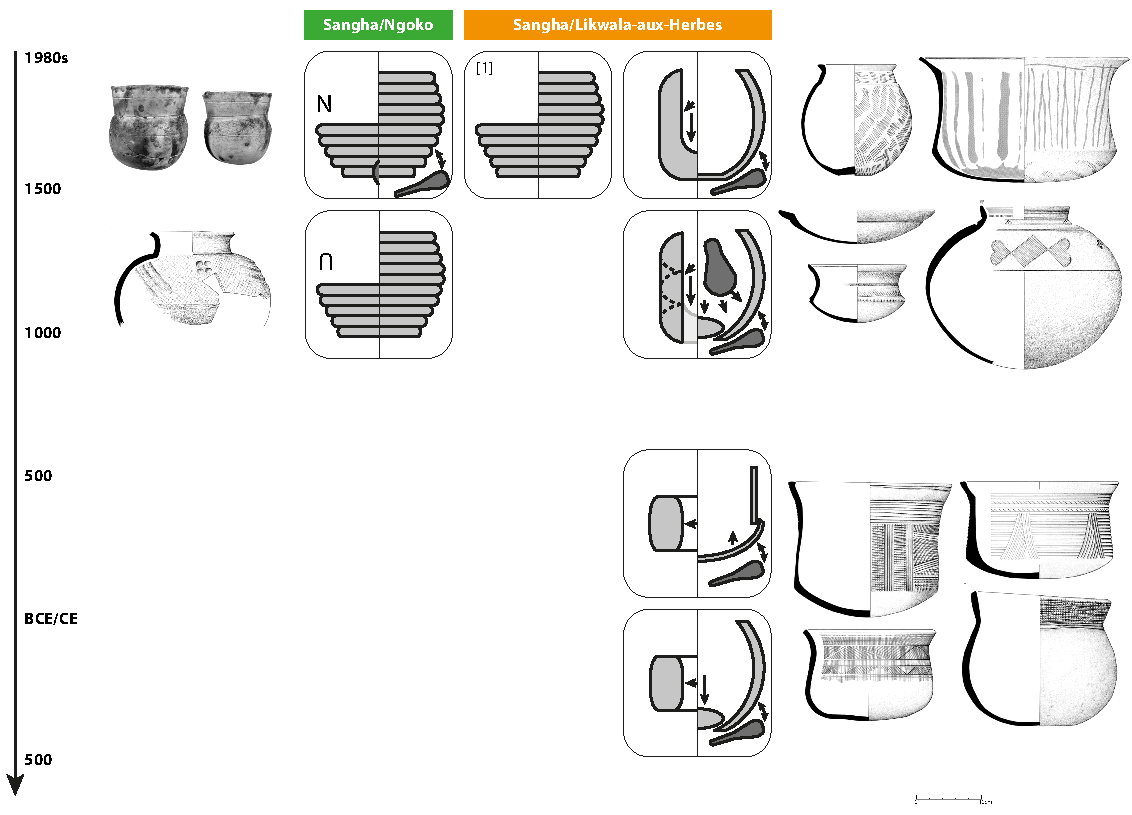
\includegraphics[width=\textwidth]{Fig_ShapingTech_Schema.pdf}
	\caption{Schematic overview of changes in primary and secondary shaping techniques along the rivers Ngoko, Sangha and Likwala-aux-Herbes throughout the past 2.000 years as reconstructed based on macro-traces and x-ray-analysis of pottery vessels. Greenish shade represents pottery styles associated with the Ngoko style tradition, while orange color represent pottery styles associated with the Pikunda-Munda style and the subsequent pottery styles related to ceramics from the Inner Congo Basin (Fig.~\ref{fig:timeslicemaps}). Ethnographic records offer insight into modern potting techniques and are either to be published elsewhere \citep{Eggert.inVorb.} or in reference to \citet[25--35; {[1]}]{MpikaNgoma.1996}. Alongside the generalized shaping techniques are representative examples of the produced vessels shows \citep[cf.][]{Seidensticker.2021e,Seidensticker.2024}}
	\label{fig:schema}
\end{figure*}

\section{Discussion}

%\subsection{\textit{Chaîne opértoire} of the Pikunda-Munda style}

A robust theoretical pillar to understanding material objects, on an individual and collective level, is the choices made during their production. The production process is best divided up into phases consisting of sequences of distinct actions and organized sets of operations to retrace the transformative trajectories that progressively alter the state of all used material resources; in the case of pottery, the raw clay and any additional temper materials \citep[3--4]{Gosselain.2018}. The integration of all those actions can be summed up using the concept of \textit{chaîne opératoire}, which has already been the predominant analytical approach to behavioral analyses in lithic technology since the 1980s \citep{Tixier.1980,Tixier.1984,Pelegrin.1988}. \textit{Chaîne opératoire} approaches enable systematic and structured comparisons between sequences of actions on an intra- and inter-community level, in Africa \citep{Gosselain.1992,Gallay.1998,Gosselain.2002,LivingstoneSmith.2007a,Mayor.2011a,MMbogori.2015,Delvoye.2016,Delvoye.2022} and elsewhere \citep[see for example][]{Manem.2008,Ard.2014,Gomart.2014,Gaffney.2020,Heitz.2023}.

Often variations in pottery technology, especially clay procurement and preparation strategies, have been interpreted rather as a result of forced adaptations to constraints imposed by the available raw materials \citep{Braun.1983,Tite.1999,Rice.2015} than a result of the socio-historical heritage of distinct potters' communities \citep{McIntosh.1995,Gosselain.2010,Roux.2017,Gosselain.2018,Roux.2019}. Pioneering studies on the socio-cultural nature and putative history of potters' behavior focused on ethno-archaeological observations \citep{Lechtman.1977}. With potting practices being learned behaviors, whose knowledge base is transferred within tight-knit social networks, mostly through kinship, the work of individual potters is interrelated through collective knowledge, tools, and materials, all together defining "communities of practice" \citep{Wenger.1998,Lave.1991a,Lave.1991,Roddick.2016}. Within such communities, knowledge is transmitted by a lived experience of participation within a social network, and actions are guided by dispositions and cultural competencies \citep{Heitz.2017a}. Training and learning, on the other hand, happen in continuous loops of applying embodied and cognitive knowledge with the use of specific tools \citep{Kuijpers.2018a}.

The results presented in this study allow reconstructing key phases within the \textit{chaîne opératoire} of potters producing Pikunda-Munda style vessels. The initial stage concerns the procurement and preparation of the raw materials. All previously studied vessel units of the Pikunda-Munda style \citep[114--120]{Seidensticker.2021e} showed a strikingly similar macroscopic fabric \citep[62 Tab.~11,69 Tab.~12]{Seidensticker.2021e}, indicating similar clay sources. The petrographic analyses presented here further corroborate the macroscopic fabrics as all studied samples of Pikunda-Munda pottery were made using clays extremely rich in sponge spicules (Fig.~\ref{fig:thinsections}A--F) that must originate from the floodplains of the rivers and smaller streams traversing the study area.

Research by \citet[148]{Gosselain.1997} showed that potters usually "satisfy themselves with a very wide spectrum of clays" and that "processing techniques are not justified by techno-functional requirements, but governed by traditions and/or individual perceptions of a particular clay's appropriateness". Thus, the observed preferences for specific clay sources and the 'recipe' in which the raw materials are handled represent chosen behaviors linked to the social identity of the potters. The findings of this study corroborate earlier observations \citep[123--124]{Seidensticker.2016b} in so far as, despite slightly varying shaping techniques and stylistic characteristics, the preference for fluvial clays among potters' communities responsible for vessels subsumed as Pikunda-Munda style is indicative of some degree of shared social identity. Especially telling is the finding from the Sangha river \citep{Seidensticker.2020}: during the Late Iron Age, fluvial clays rich in sponge spicules were not used by potters of the younger Ngoko style tradition (greenish colored styles in Fig.~\ref{fig:timeslicemaps}; \ref{fig:thinsections}:J--L; \ref{fig:PIK87_1-2_3_macrotraces}; \ref{fig:PIK87_1_macrotraces}; \ref{fig:sangahtypes}:13--21; and \ref{fig:schema}), while potters producing other contemporaneous styles such as Ngombe, Ebambe, Epena, or Mobaka (orange-brownish colored styles in Fig.~\ref{fig:timeslicemaps}; \ref{fig:thinsections}:G--I; \ref{fig:NGO87_102_27_macrotraces}; \ref{fig:NGO87_102_28-29_macrotraces}; \ref{fig:sangahtypes}:10--12 \& 22--26; and \ref{fig:schema}) were still relying exclusively on fluvial clays, similar to Pikunda-Munda potters' earlier. This further underlines that potters of the Ngoko style tradition, whose vessels are shaped by coiling \citep[Figs.~\ref{fig:PIK87_1-2_3_macrotraces} and \ref{fig:PIK87_1_macrotraces};][53--54 Fig.~16B, 72 Tab.~13]{Seidensticker.2021e}, similar to the modern pottery (Fig.~\ref{fig:PIK87_501_2_macrotraces}), do not share any aspect of their potting behavior with preceding communities. On the other hand, potters along the lower Sangha, as well as the Likwala-aux-Herbes river, pertained the preference for fluvial clays (Fig.~\ref{fig:thinsections}G--I). River clays are also the prevalent source used in the western parts of the Inner Congo Basin, and pottery dating into the Late Iron Age along the lower Sangha and Likwala-aux-Herbes river are, with varying degrees, stylistically related to styles of the West tradition of the Equator-Co style tradition \citep[221--222 Fig.~4]{Wotzka.1995}. Future research will test to what degree the preference for fluvial clays is also a hallmark of the Equator-Co style tradition.

Additionally, this study provides further insight into the primary and secondary shaping techniques of Pikunda-Munda style pottery. While earlier research \citep[47--51 Fig.~13,69--73]{Seidensticker.2021e} already suggested that Pikunda-Munda vessels were produced through drawing, this study could further specify the technique: Pikunda-Munda potters produced their vessels through the drawing of a ring technique, and bases were either closed with additional clay or a separately shaped slab bottom (Fig.~\ref{fig:schema}).

%\subsection{What happens after the Pikunda-Munda pottery?}

While there are no indications for the origin of the Pikunda-Munda pottery and its distinct \textit{chaîne opératoire}, the exact cause for its disappearance is equally unclear. The youngest feature yielding Pikunda-Munda style pottery is a pit connected to an open bowl furnace or smith's hearth at Munda dating into the third to sixth century CE \citep[335--339 Fig.~170]{Seidensticker.2021e}. The next youngest pottery style identified along the lower Sangha river is the Ngombe style \citep[Fig.~\ref{fig:timeslicemaps};][125--128]{Seidensticker.2021e}, recently dated into the late twelfth to mid thirteenth century CE \citep[Tab.~2: RICH-30864]{Seidensticker.2024}. The vessels of the Ngombe style show substantial stylistic similarities to the Longa and Mbandaka pottery of the Inner Congo Basin \citep[121--128,139--143]{Wotzka.1995}. The pottery from Ngombe is made of fluvial clays rich in sponge spicules \citep{Seidensticker.2020} and at least the big globular vessel is shaped via drawing of superimposed rings \citep[Figs.~\ref{fig:NGO87_102_27_macrotraces} and \ref{fig:NGO87_102_28-29_macrotraces};][52--53 Fig.~15]{Seidensticker.2021e}. Worth mentioning is the presence of carinated bowls within the Ngombe style (Fig.~\ref{fig:NGO87_102_27_macrotraces} and \ref{fig:sangahtypes}.10), strikingly similar to the characteristic carinated bowls of the Longa pottery from the Inner Congo Basin \citep[121--128]{Wotzka.1995}. The main vessel shape, with its flared rims, concave upper parts, and pronounced carinations leading to round bases \citep[197 Fig.~94.1--2]{Seidensticker.2021e} are the only putative typological remnant one might consider to discuss in terms of heritage of the Pikunda-Munda bowls.

Along the Likwala-aux-Herbes river, pottery production is only attested for from the sixteenth century CE onward again (Fig.~\ref{fig:timeslicemaps}), as represented by the Ebambe style \citep[Fig.~\ref{fig:sangahtypes}.22--23;][131--136]{Seidensticker.2021e}. Vessels of that style are very similar to the modern Epena style \citep[Fig.~\ref{fig:sangahtypes}.25--26;][137--141]{Seidensticker.2021e}, and both styles are produced exclusively using fluvial clays as well \citep{Seidensticker.2020}. Regarding shaping techniques, preliminary research found that vessels of both styles share features indicative of the drawing of a ring or drawing of superimposed rings technique \citep[Fig.~\ref{fig:schema};][55--57 Fig.~17--18]{Seidensticker.2021e}. Of particular interest in terms of the 'heritage' of the Pikunda-Munda pottery among modern pottery in the region is the Mobaka pottery style \citep[141--144]{Seidensticker.2021e}. The defining feature of this style are carinated bowls of seemingly the same basic shape as in the Pikunda-Munda group \citep[Fig.~\ref{fig:sangahtypes}.24;][142 Fig.~63.1,64]{Seidensticker.2021e}. At this stage, it remains unfortunately unclear why modern potters' producing the Mobaka style bowls choose this particular shape.

Further upstream of Pikunda (Fig.~\ref{fig:map}), pottery production commences again from the thirteenth century onward (Fig.~\ref{fig:timeslicemaps}). The stylistic characteristics are substantially different, and ceramics are part of the Ngoko style tradition consisting of five successive style groups: Mandombe, Konda, Ouesso, Pandama, and Mbenja \citep[Fig.~\ref{fig:sangahtypes}.13--21;][145--162]{Seidensticker.2021e}. Besides globular pots being the dominant vessel shape among these styles, they all have been produced using clays void of sponge spicules \citep[Fig.~\ref{fig:thinsections}.J--K;][]{Seidensticker.2020}. Preliminary research on archaeological finds \citep[Fig.~\ref{fig:PIK87_1-2_3_macrotraces}--\ref{fig:PIK87_1_macrotraces};][53--54 Fig.~16B]{Seidensticker.2021e} as well as ethnographic records and ceramic vessel (Fig.~\ref{fig:PIK87_501_2_macrotraces}) indicate that coiling is the defining shaping technique within the Ngoko style tradition (Fig.~\ref{fig:schema}). Thus, the styles of the Ngoko style tradition are considered distinct, potentially originating further upstream along the Sangha and Ngoko/Dja rivers in south-east Cameroon. 

%\subsection{Integration in pottery traditions}

Ethnographic research at Ikenge on the Ruki river (Fig.~\ref{fig:map}), the foremost potters village in the Inner Congo Basin, describes a \textit{chaîne opératoire} in which the primary shaping or roughing-out starts with hollowing out of a lump \citep{Eggert.1980c}. The pierced lump, now practically converted into a ring of clay, is further shaped by drawing, and additional clay is added to shape the base. This process involves pounding of the base on a flat surface and paddling of the outside. Among modern potters along the rivers Tshuapa, Busira, and Maringa, this general approach is slightly altered as a mat is used as pad during the pounding, leaving diagnostic markings \citep[188,196--197]{Wotzka.1995}. Preliminary research on the shaping techniques of vessels dating into the Early Iron Age in the Inner Congo basin revealed features more related to a 'pure' drawing of a lump technique, as there are no signs of any addition of clay or separate forming techniques being used for the bases compared to the upper parts. Thus, the distinct drawing of a ring technique employed by Pikunda-Munda potters has no immediate connection to contemporaneous communities further east, as far as current research goes. But, in the north-eastern Congo Basin, drawing of a ring technique is practices \citep[110,115]{LivingstoneSmith.2017}. There, pottery of the early and middle phase has been shaped via this technique. The region saw a substantial change in shaping techniques as all pottery pertaining to the Late Iron Age is produced via pounding in a concave mold \citep[111,115]{LivingstoneSmith.2017}. In the northern Congo Basin, along the Ubangi river, the \textit{chaîne opératoire} of only the youngest ceramics could be identified. Along the middle part of the river, coiling has been documented, while further north, already in the northern Savannas, pounding in a concave mold is practiced \citep[55--60 Fig.~19--20,73]{Seidensticker.2021e}. The current patchwork of data on pottery technology in the Congo Basin and its evolvement through time prevents any integration of the \textit{chaîne opératoire} of Pikunda-Munda potters into a wider framework.

%\subsection{Ramifications for debate on Bantu-Expansion}

The end of the Pikunda-Munda pottery style in the fifth to sixth century CE corresponds with the supra-regional setback in human activity, which was first described on a regional level \citep{Oslisly.1998}, and firmly established independently by \citet{deSaulieu.2021a} and \citet{Seidensticker.2021}. While at the supra-regional scale a state of 'low activity' with relic populations \citep[cf.][Fig.~S4]{Seidensticker.2021} can be identified, in the western Congo Basin, the region of the Pikunda-Munda style pottery, a complete hiatus, and end of the tradition of Pikunda-Munda potters' communities must be presumed. The pottery inventories themselves offer no signs that any distinct traits of the Pikunda-Munda potters' knowledge persisted, as no subsequent pottery shows any reminiscence of this older pottery. The mentioned similarities in terms of clay sourcing and preparation strategies, specifically the universal sourcing of fluvial clays that are used without tempering, are no characteristic of the Pikunda-Munda pottery alone. With complete \textit{chaînes opératoires} for ceramic production in the Congo Basin largely missing, it must remain a subject of future research what the diagnostic features of the 'recipe' of Pikunda-Munda potters were. A viable candidate for a unique characteristic of their \textit{chaîne opératoire} might be the drawing of a ring technique with slab bottoms, which is not present in any of the subsequent pottery types. But many unknowns remain, especially in the way in which the Equator-Co style tradition \citep{Wotzka.1995} constitutes the---at least somewhat 'stable'---backbone of a genealogical network for trans-generational knowledge transfer among potters communities in the wider region. But follow-up examinations \citep[193--204]{Seidensticker.2021e} and a novel radiocarbon date \citep[Tab.~2: RICH-30867]{Seidensticker.2024} raise chronological issues that need to be resolved before claiming long-lasting continuities spanning the period of 'low activity'.

Despite the regional scope of this study, it highlights a distinctiveness of archaeological research, which research focused on retracing of modern languages or genetic compositions of equally modern communities is incapable of, namely the detection of disappearances of items of material culture accompanied by discontinuities in the genealogical networks of knowledge transfer. While the prevailing hypotheses of the 'Bantu-Expansion' have been critiqued for many decades \citep{deMaret.1989,Robertson.2000,Eggert.2005,Eggert.2016a}, 'discontinuity' has not been a focal point of the debate yet, despite the latest set of proposed models \citep{Bostoen.2015,Grollemund.2015,Grollemund.2023,Koile.2022} necessitate profound continuities. The statistical approaches used to reconstruct past languages from modern datasets are unable to detect contact induced change \cite[86]{Eggert.2016a} or inter-community knowledge-transfer as well as estimating the rates of speciation and extinction reliably \citep{Pagel.2020}. The reliance on a single strain of material culture, namely pottery production, is a further issue. Not only is any generalization that is based on a single component of the material culture of prehistoric communities inherently insufficient, but the level of research on many facets of the prehistoric communities producing and distributing ceramics in Central Africa, like their networks of trade or trans-communal knowledge transfer among others, is only in its infancy. The available debate on the 'Bantu-Expansion' constitutes discipline-specific "procedural puzzles" \citep[88]{Eggert.2016a} devoted to the "separate histories" materialized in modern languages, population genetics \citep{FortesLima.2024}, and items of material culture without any ability of deducing the immaterial nature of non-written languages through material traces \citep[85]{Eggert.2016a}. The current view in which the purely linguistic term 'Bantu' has been transformed to refer "indiscriminately to language, culture, society, and race" \citep[302]{Eggert.2005} must be scrutinized in-depth and untangled where necessary to avoid the circular reasoning plaguing the debate \citep{Ehret.1973,Phillipson.1976,Phillipson.1976b,Phillipson.1977a,Heine.1977,Bostoen.2015,Grollemund.2015,Grollemund.2023,Koile.2022}.

\section{Conclusions}

This paper presents novel data on the pottery of the Pikunda-Munda style, which is among the oldest ceramics found in the western Congo Basin, dating from the second century BCE to the fifth/sixth century CE. It thus emerges around 200 years after the Imbonga pottery group, appearing further east to the most ancient pottery in the Congo Basin \cite[Fig.~\ref{fig:timeslicemaps};][59--68]{Wotzka.1995}. Moreover, Pikunda-Munda pottery shares certain characteristics with contemporaneous ceramics of the Inner Congo Basin \citep[107 Ftn.~4]{Wotzka.1995}. Besides stylistic similarities, such as the usage of similar tools for decorating and preferences of motives, including rocker-stamping with a comb \citep[118 Tab.~14]{Seidensticker.2021e}, Pikunda-Munda potters also used fluvial clays rich in sponge spicules without the addition of any temper agents. What sets Pikunda-Munda vessels apart are the shape of the vessels: its carinated bowls with round bases are unique within the Early Iron Age in the Congo Basin. All its characteristics vanish after the fifth to sixth century CE, and they leave little to no trace in any other subsequent pottery nearby. The next youngest pottery in the western Congo Basin, preceding the Pikunda-Munda style, can only be dated to the twelfth century CE at the earliest \citep[Tab.~2: RICH-30864]{Seidensticker.2024}, leaving a ~500 year gap with no pottery finds---even tentatively---being dated into (Fig.~\ref{fig:timeslicemaps}A).

The present research, while still in its infancy, shows that the focus on stylistic changes seen within the archaeological research of the region \citep{Wotzka.1995,Seidensticker.2021e} is only scratching the surface. Vessel morphology and decorations depict changes in fashion trends, while the detailed technical analyses shown here enable a reconstruction of decisions made by potters that tie together communities of practices.

\begin{acknowledgements}
First and foremost, I want to thank Manfred K. H. Eggert for granting me access to the finds from his project and supporting the research. This research was funded by the Fonds Wetenschappelijk Onderzoek - Vlaanderen (FWO; 1287922N). The Commissie Wetenschappelijk Onderzoek (CWO) of Ghent University funded the preparation of an initial set of thin-sections. Many thanks goes to Garin Cael and Alexandre Livingstone Smith for preparing the radiographs at the Royal Museum for Central Africa (RMCA) Tervuren. Further, I would also like to thank the two reviewers, whose comments improved the paper very much.

All data, images, and computer code generated during this research are available here: \url{https://github.com/dirkseidensticker/PikundaMunda_DissapearingPotteryTraditions_AAR}.
\end{acknowledgements}

\bibliographystyle{spbasic}
\bibliography{references.bib}

\end{document}
